%==============================================================================
% Tento soubor použijte jako základ
% This file should be used as a base for the thesis
% Autoři / Authors: 2008 Michal Bidlo, 2022 Jaroslav Dytrych
% Kontakt pro dotazy a připomínky: sablona@fit.vutbr.cz
% Contact for questions and comments: sablona@fit.vutbr.cz
%==============================================================================
% kódování: UTF-8 (zmena prikazem iconv, recode nebo cstocs)
% encoding: UTF-8 (you can change it by command iconv, recode or cstocs)
%------------------------------------------------------------------------------
% zpracování / processing: make, make pdf, make clean
%==============================================================================
% Soubory, které je nutné upravit nebo smazat: / Files which have to be edited or deleted:
%   projekt-20-literatura-bibliography.bib - literatura / bibliography
%   projekt-01-kapitoly-chapters.tex - obsah práce / the thesis content
%   projekt-01-kapitoly-chapters-en.tex - obsah práce v angličtině / the thesis content in English
%   projekt-30-prilohy-appendices.tex - přílohy / appendices
%   projekt-30-prilohy-appendices-en.tex - přílohy v angličtině / appendices in English
%==============================================================================
% \documentclass[]{fitthesis} % bez zadání - pro začátek práce, aby nebyl problém s překladem
%\documentclass[english]{fitthesis} % without assignment - for the work start to avoid compilation problem
%\documentclass[zadani]{fitthesis} % odevzdani do IS VUT a/nebo tisk s barevnými odkazy - odkazy jsou barevné
%\documentclass[english,zadani]{fitthesis} % for submission to the IS VUT and/or print with color links - links are color
%\documentclass[zadani,print]{fitthesis} % pro černobílý tisk - odkazy jsou černé
% \documentclass[english,zadani,print]{fitthesis} % for the black and white print - links are black
% \documentclass[zadani,cprint]{fitthesis} % pro barevný tisk - odkazy jsou černé, znak VUT barevný
\documentclass[english,zadani,cprint]{fitthesis} % for the print - links are black, logo is color
% * Je-li práce psaná v anglickém jazyce, je zapotřebí u třídy použít 
%   parametr english následovně:
%   If thesis is written in English, it is necessary to use 
%   parameter english as follows:
%      \documentclass[english]{fitthesis}
% * Je-li práce psaná ve slovenském jazyce, je zapotřebí u třídy použít 
%   parametr slovak následovně:
%   If the work is written in the Slovak language, it is necessary 
%   to use parameter slovak as follows:
%      \documentclass[slovak]{fitthesis}
% * Je-li práce psaná v anglickém jazyce se slovenským abstraktem apod., 
%   je zapotřebí u třídy použít parametry english a enslovak následovně:
%   If the work is written in English with the Slovak abstract, etc., 
%   it is necessary to use parameters english and enslovak as follows:
%      \documentclass[english,enslovak]{fitthesis}

% Základní balíčky jsou dole v souboru šablony fitthesis.cls
% Basic packages are at the bottom of template file fitthesis.cls
% zde můžeme vložit vlastní balíčky / you can place own packages here


% Pro seznam zkratek lze využít balíček Glossaries - nutno odkomentovat i níže a při kompilaci z konzoly i v Makefile (plnou verzi pro Perl, nebo lite)
% The Glossaries package can be used for the list of abbreviations - it is necessary to uncomment also below. When compiling from the console also in the Makefile (full version for Perl or lite)
%\usepackage{glossaries}
%\usepackage{glossary-superragged}
%\makeglossaries 

% Nastavení cesty k obrázkům
% Setting of a path to the pictures
%\graphicspath{{obrazky-figures/}{./obrazky-figures/}}
%\graphicspath{{obrazky-figures/}{../obrazky-figures/}}

%---rm---------------
\renewcommand{\rmdefault}{lmr}%zavede Latin Modern Roman jako rm / set Latin Modern Roman as rm
%---sf---------------
\renewcommand{\sfdefault}{qhv}%zavede TeX Gyre Heros jako sf
%---tt------------
\renewcommand{\ttdefault}{lmtt}% zavede Latin Modern tt jako tt

% vypne funkci šablony, která automaticky nahrazuje uvozovky,
% aby nebyly prováděny nevhodné náhrady v popisech API apod.
% disables function of the template which replaces quotation marks
% to avoid unnecessary replacements in the API descriptions etc.
\csdoublequotesoff

\usepackage{dirtree}
\usepackage{url}

% =======================================================================
% balíček "hyperref" vytváří klikací odkazy v pdf, pokud tedy použijeme pdflatex
% problém je, že balíček hyperref musí být uveden jako poslední, takže nemůže
% být v šabloně
% "hyperref" package create clickable links in pdf if you are using pdflatex.
% Problem is that this package have to be introduced as the last one so it 
% can not be placed in the template file.
\ifWis
\ifx\pdfoutput\undefined % nejedeme pod pdflatexem / we are not using pdflatex
\else
  \usepackage{color}
  \usepackage[unicode,colorlinks,hyperindex,plainpages=false,pdftex]{hyperref}
  \definecolor{hrcolor-ref}{RGB}{223,52,30}
  \definecolor{hrcolor-cite}{HTML}{2F8F00}
  \definecolor{hrcolor-urls}{HTML}{092EAB}
  \hypersetup{
	linkcolor=hrcolor-ref,
	citecolor=hrcolor-cite,
	filecolor=magenta,
	urlcolor=hrcolor-urls
  }
  \def\pdfBorderAttrs{/Border [0 0 0] }  % bez okrajů kolem odkazů / without margins around links
  \pdfcompresslevel=9
\fi
\else % pro tisk budou odkazy, na které se dá klikat, černé / for the print clickable links will be black
\ifx\pdfoutput\undefined % nejedeme pod pdflatexem / we are not using pdflatex
\else
  \usepackage{color}
  \usepackage[unicode,colorlinks,hyperindex,plainpages=false,pdftex,urlcolor=black,linkcolor=black,citecolor=black]{hyperref}
  \definecolor{links}{rgb}{0,0,0}
  \definecolor{anchors}{rgb}{0,0,0}
  \def\AnchorColor{anchors}
  \def\LinkColor{links}
  \def\pdfBorderAttrs{/Border [0 0 0] } % bez okrajů kolem odkazů / without margins around links
  \pdfcompresslevel=9
\fi
\fi
% Řešení problému, kdy klikací odkazy na obrázky vedou za obrázek
% This solves the problems with links which leads after the picture
\usepackage[all]{hypcap}


% Informace o práci/projektu / Information about the thesis
%---------------------------------------------------------------------------
\projectinfo{
  %Prace / Thesis
  project={BP},            %typ práce BP/SP/DP/DR  / thesis type (SP = term project)
  year={2023},             % rok odevzdání / year of submission
  date=\today,             % datum odevzdání / submission date
  %Nazev prace / thesis title
  title.cs={Simulace procházení webu člověkem},  % název práce v češtině či slovenštině (dle zadání) / thesis title in czech language (according to assignment)
  title.en={Human web browsing simulation}, % název práce v angličtině / thesis title in english
  %title.length={14.5cm}, % nastavení délky bloku s titulkem pro úpravu zalomení řádku (lze definovat zde nebo níže) / setting the length of a block with a thesis title for adjusting a line break (can be defined here or below)
  %sectitle.length={14.5cm}, % nastavení délky bloku s druhým titulkem pro úpravu zalomení řádku (lze definovat zde nebo níže) / setting the length of a block with a second thesis title for adjusting a line break (can be defined here or below)
  %dectitle.length={14.5cm}, % nastavení délky bloku s titulkem nad prohlášením pro úpravu zalomení řádku (lze definovat zde nebo níže) / setting the length of a block with a thesis title above declaration for adjusting a line break (can be defined here or below)
  %Autor / Author
  author.name={Jáchym},   % jméno autora / author name
  author.surname={Doležal},   % příjmení autora / author surname 
  %author.title.p={Bc.}, % titul před jménem (nepovinné) / title before the name (optional)
  %author.title.a={Ph.D.}, % titul za jménem (nepovinné) / title after the name (optional)
  %Ustav / Department
  department={UIFS}, % doplňte příslušnou zkratku dle ústavu na zadání: UPSY/UIFS/UITS/UPGM / fill in appropriate abbreviation of the department according to assignment: UPSY/UIFS/UITS/UPGM
  % Školitel / supervisor
  supervisor.name={Radek},   % jméno školitele / supervisor name 
  supervisor.surname={Hranický},   % příjmení školitele / supervisor surname
  supervisor.title.p={Ing.},   %titul před jménem (nepovinné) / title before the name (optional)
  supervisor.title.a={Ph.D.},    %titul za jménem (nepovinné) / title after the name (optional)
  % Klíčová slova / keywords
  keywords.cs={Simulace lidského chování, Transformátory, OpenAI, Webové technologie, Technologický pokrok, Velké jazykové modely, Automatizace webových stránek}, % klíčová slova v českém či slovenském jazyce / keywords in czech or slovak language
  keywords.en={Human behavior simulation, Transformers, OpenAI, Web technologies, Technological advancements, Large Language Models, Website automation}, % klíčová slova v anglickém jazyce / keywords in english
  %keywords.en={Here, individual keywords separated by commas will be written in English.},
  % Abstrakt / Abstract
  abstract.cs={Tato práce představuje slibný nástroj pro automatizovanou webovou navigaci a plnění specifických cílů podle rozhodnutí daných velkým jazykovým modelem, který používá aktuální informace z dané stránky. Výsledky simulátoru s modelem GPT 4 Turbo demonstrují efektivitu tohoto nástroje, který dosahuje úspěšnosti přes 80\% v dokončování předem definovaných cílů. Výsledky dokazují použiteljnost tohoto nástroje v reálných případech užití.}, % abstrakt v českém či slovenském jazyce / abstract in czech or slovak language
  abstract.en={
This work introduces a promising tool for automated web
navigation and achieving specific goals based on decisions made by a Large Language Model using information from a current page. The results of the simulator with model GPT 4 Turbo demonstrate the tool's effectiveness, achieving over 80\% success in completing predefined goals. The results show the usability of this tool in real use cases.}, % abstrakt v anglickém jazyce / abstract in english
  %abstract.en={An abstract of the work in English will be written in this paragraph.},
  % Prohlášení (u anglicky psané práce anglicky, u slovensky psané práce slovensky; u projektové praxe lze zakomentovat) / Declaration (for thesis in english should be in english; for project practice can be commented out)
  declaration={Prohlašuji, že jsem tuto bakalářskou práci vypracoval samostatně pod vedením pana Ing. Hranického Ph.D.
Uvedl jsem všechny literární prameny, publikace a další zdroje, ze kterých jsem čerpal.},
  %declaration={I hereby declare that this Bachelor's thesis was prepared as an original work by the author under the supervision of Mr. X
% The supplementary information was provided by Mr. Y
% I have listed all the literary sources, publications and other sources, which were used during the preparation of this thesis.},
  % Poděkování (nepovinné, nejlépe v jazyce práce; nechcete-li, zakomentujte pro skrytí nadpisu) / Acknowledgement (optional, ideally in the language of the thesis; comment out for hiding including heading)
  acknowledgment={I would like to extend my heartfelt gratitude to my supervisor, Ing. Radek Hranický Ph.D., for his invaluable guidance and insights throughout this project. His encouragement helped me to push this project forward. I would also like to express my gratitude to my family and girlfriend, whose constant support was essential for completing this project.},
  %acknowledgment={Here it is possible to express thanks to the supervisor and to the people which provided professional help
%(external submitter, consultant, etc.).},
  % Rozšířený abstrakt (cca 3 normostrany) - lze definovat zde nebo níže / Extended abstract (approximately 3 standard pages) - can be defined here or below
  %extendedabstract={Do tohoto odstavce bude zapsán rozšířený výtah (abstrakt) práce v českém (slovenském) jazyce.},
  %extabstract.odd={true}, % Začít rozšířený abstrakt na liché stránce? / Should extended abstract start on the odd page?
  %faculty={FIT}, % FIT/FEKT/FSI/FA/FCH/FP/FAST/FAVU/USI/DEF
  faculty.cs={Fakulta informačních technologií}, % Fakulta v češtině - pro využití této položky výše zvolte fakultu DEF / Faculty in Czech - for use of this entry select DEF above
  faculty.en={Faculty of Information Technology}, % Fakulta v angličtině - pro využití této položky výše zvolte fakultu DEF / Faculty in English - for use of this entry select DEF above
  department.cs={Ústav informačních systémů}, % Ústav v češtině - pro využití této položky výše zvolte ústav DEF nebo jej zakomentujte / Department in Czech - for use of this entry select DEF above or comment it out
  department.en={Institute of Information Systems} % Ústav v angličtině - pro využití této položky výše zvolte ústav DEF nebo jej zakomentujte / Department in English - for use of this entry select DEF above or comment it out
  
}

% Rozšířený abstrakt (cca 3 normostrany) - lze definovat zde nebo výše / Extended abstract (approximately 3 standard pages) - can be defined here or above
\extendedabstract{Cílem této práce bylo vytvořit simulátor schopný napodobit člověka při procházení webu. Při využití technologií, jakou jsou velké jazykové modely, zejména modelu GPT-4 Turbo od společnosti OpenAI, se tato práce snaží překročit propast v technologiích umožnující simulaci lidského chování při procházení webu. Jazykové modely i přes svá omezení, jakou jsou omezené kontextové okna a výskyt halucinací, představují slibnou technologii pro simulaci lidského chování díky schopnosti rozumět přirozené lidské řeči a možnosti modelování lidských rozhodnutí.

Výsledkem této práce je simulátor, který simuluje lidské interakce na webových stránkach, založené na textové specifikaci cíle a webové stránky. Tento nástroj by mohl najít uplantění v mnoha oblastech, od testování webových stránek až po rozpoznávání webových botů a vývoj aplikací poháněné umělou inteligencí. 

Simulátor představen v této práci umožňuje plnění předem zadaného cíle na dané webové stránce. V jádru simulátoru se nachází jazykový model, který který vybírá vhodné akce pro splnění daného cíle na základě předchozích akcí a aktuálních informacích o dané stránce. Pomocí využití knihoven LangChain a Selenium je aplikace vytvořena a schopna plnění širokého množství cílů na různých webových stránkách. Cíle se mohou týkat webové navigace a získávání dat z webových stránek. 

Závěry experimentů v této práci ukázaly, že simulátor s modelem GPT-4 Turbo dosahuje úspěšnosti nad 80\%. Současně výsledky při porovnání s lidskou navigací na webu prokázali shodu rozhodování mezi simulátorem a člověkem. Závěr práce naznačuje, jak by mohl být tento nástroj využit v realných případech užití a zdůrazňují potenciál pro další vývoj.

Budoucí výzkum by se mohl zaměřit na testování simulátoru na širší a detailnější škále webů a srovnání výsledků s detailnější datovou sadou lidské interakce na webu. Dále závěr práce mluví o možnosti rozšíření simulátoru kde by byl schopný vytvářet své vlastní cíle na základě definovaného profila uživatele.}
% Začít rozšířený abstrakt na liché stránce? / Should extended abstract start on the odd page?
\extabstractodd{true}

% nastavení délky bloku s titulkem pro úpravu zalomení řádku - lze definovat zde nebo výše / setting the length of a block with a thesis title for adjusting a line break - can be defined here or above
%\titlelength{14.5cm}
% nastavení délky bloku s druhým titulkem pro úpravu zalomení řádku - lze definovat zde nebo výše / setting the length of a block with a second thesis title for adjusting a line break - can be defined here or above
%\sectitlelength{14.5cm}
% nastavení délky bloku s titulkem nad prohlášením pro úpravu zalomení řádku - lze definovat zde nebo výše / setting the length of a block with a thesis title above declaration for adjusting a line break - can be defined here or above
%\dectitlelength{14.5cm}

% řeší první/poslední řádek odstavce na předchozí/následující stránce
% solves first/last row of the paragraph on the previous/next page
\clubpenalty=10000
\widowpenalty=10000

% checklist
\newlist{checklist}{itemize}{1}
\setlist[checklist]{label=$\square$}

% Kompilace po částech (rychlejší, ale v náhledu nemusí být vše aktuální)
% Compilation piecewise (faster, but not all parts in preview will be up-to-date)
% Další informace viz / For more information see https://www.overleaf.com/learn/latex/Multi-file_LaTeX_projects
% \usepackage{subfiles}

% Nechcete-li, aby se u oboustranného tisku roztahovaly mezery pro zaplnění stránky, odkomentujte následující řádek / If you do not want enlarged spacing for filling of the pages in case of duplex printing, uncomment the following line
% \raggedbottom

\begin{document}
  % Vysazeni titulnich stran / Typesetting of the title pages
  % ----------------------------------------------
  \maketitle
  % Obsah
  % ----------------------------------------------
  \setlength{\parskip}{0pt}

  \setcounter{tocdepth}{1}
  

  {\hypersetup{hidelinks}\tableofcontents}
  
  % Seznam obrazku a tabulek (pokud prace obsahuje velke mnozstvi obrazku, tak se to hodi)
  % List of figures and list of tables (if the thesis contains a lot of pictures, it is good)
  % \ifczech
  %   \renewcommand\listfigurename{Seznam obrázků}
  % \fi
  % \ifslovak
  %   \renewcommand\listfigurename{Zoznam obrázkov}
  % \fi
  % {\hypersetup{hidelinks}\listoffigures}
  
  \ifczech
    \renewcommand\listtablename{Seznam tabulek}
  \fi
  \ifslovak
    \renewcommand\listtablename{Zoznam tabuliek}
  \fi
  % {\hypersetup{hidelinks}\listoftables}

  % Seznam zkratek / List of abbreviations
  %\ifczech
  %  \renewcommand*\glossaryname{Seznam zkratek}%
  %  \renewcommand*\entryname{Zkratka}
  %  \renewcommand*\descriptionname{Význam}
  %\fi
  %\ifslovak
  %  \renewcommand*\glossaryname{Zoznam skratiek}%
  %  \renewcommand*\entryname{Skratka}
  %  \renewcommand*\descriptionname{Význam}
  %\fi
  %\ifenglish
  %  \renewcommand*\glossaryname{List of abbreviations}%
  %  \renewcommand*\entryname{Abbreviation}
  %  \renewcommand*\descriptionname{Meaning}
  %\fi
  % Definice zkratek - z textu se odkazují např. \Gls{TF–IDF}
  % Definition of abbreviations - referred from the text e.g. \Gls{TF–IDF}
  %\newglossaryentry{TF–IDF}
  %{
  %  name={TF–IDF},
  %  description={Term Frequency-Inverse Document Frequency}
  %}
  % 
  %\setglossarystyle{superragged}
  %\printglossaries


  \ifODSAZ
    \setlength{\parskip}{0.5\bigskipamount}
  \else
    \setlength{\parskip}{0pt}
  \fi

  % vynechani stranky v oboustrannem rezimu
  % Skip the page in the two-sided mode
  \iftwoside
    \cleardoublepage
  \fi

  % Text prace / Thesis text
  % ----------------------------------------------
  \ifenglish
    \chapter{Introduction}

The merits of technological advancements were usually the automation of tasks too repetitive for humans. With advancements in Machine Learning and AI models, further opportunities for automation are possible. Websites typically have unique structures based on their purpose. Even two given websites of similar categories have completely different structures. Therefore, it is a challenging task to create an algorithm that would orientate inside such a website. To create a simulator that can simulate humans browsing a website, choosing a~technology that can analyze text and create action based on the given technology is crucial. The tasks of NLP and NLU are among the fastest branches in computer science. The invention of Transformers in 2017 \cite{attention} sped up the field advancements. Nowadays, many influential models are capable of understanding language and simulating humans. 

This thesis takes the creation of a simulator that can simulate human web browsing. The task of simulating human behavior is a very complex one. The most complex model nowadays is GPT-4 created by OpenAI, a large language model trained on a big chunk of the internet. The model has the best understanding of humans yet created. LLM models are the most promising technology created for simulating human behavior. However, the LLMs come with new challenges. With their limited context and occurrence of hallucinations, it is sometimes challenging for them to complete given goals. Furthermore, the models are moderately slow. The ideal approach is to use models for tasks that are otherwise extremely challenging. The thesis will provide a detailed view of how to design and implement such a~simulator. Additionally, it will also explore the history and mechanisms of LLM technology. 

The motivation for this research is driven by the rapid advancement in web technologies and the complexity of human-web interactions. In today's digital-centric world, understanding and replicating human behavior in web environments is increasingly important for enhancing user experience and developing efficient web-based services. This study addresses the gap in technologies and methodologies for accurately simulating human browsing behavior. By leveraging Large Language Models (LLMs) as the decision-making core, supplemented by other components, this research aims to develop a simulator that closely mirrors human interactions with web pages.

This study's significance lies in its potential to advance the field of human-computer interaction, offering insights and practical solutions for web design, usability, web testing, web bot detection, and AI development. While focused specifically on web browsing behavior, the implications of this research extend to broader applications in digital behavior analysis and AI ethics.

The proposed tool aims to create a simulator capable of web navigation and retrieval based on a textual specification of a goal on a previously unvisited website. This work shows the usability of LLms in human simulation tasks on the web. The work can help to create an advanced tool for web testing, or it can be used in different use cases for human simulation on the web or automatized web navigation and data retrieval. The results of the experiments \ref{experiment} show the high capability of the simulator with an accuracy, averaging 82.1\% success rate with the best model and showing similarities with human web navigation.

Chapter \ref{rw} discusses the related work to this thesis, analyzing the previous approaches and comparing them with the proposed approach by this thesis. Chapter \ref{tb} presents the technical and historical background of LLMs and their overview. Furthermore, Chapter \ref{tech} describes both technologies that will be used for the implementation of the simulator and technology used for web control or the integration of LLMs into applications. Chapter \ref{da} explains the components of a simulator proposed in this thesis. The chapter describes the scope of the work and explains the whole architecture of the simulator. The following Chapter \ref{imp} describes each component from the implementation perspective. Chapter \ref{experiment} shows ways in which the tool was tested and presents the achieved results. Lastly, Chapter \ref{con} summarizes the findings of this work and future development.    

% add prinos peace odstavec 2 kde vysvtlim prinosy peace co jsem navrhl k cemu je to dobre a uzitecne

% samostatny odstavec an zminku experimentalnich vysledku zhodnoceni, podarilo see mi zjistit ze metodologie co jsem pouzil k ucelu je pouzitlna ... a zminit konkretni vysledky ciselne vysledky experiment bla bla

\chapter{Related work}
\label{rw}

This chapter will briefly discuss existing approaches for simulating human behavior on the web and human simulation techniques in general. The following text should provide a better context of the field and a better starting point for the thesis. Because combining human simulation and web browsing is not a common thesis, few papers discuss both topics. However, The works still have relevant information about web agents and human simulation.

\section{Web prediction and web agents}

Web bot development has always been an ongoing 'arms race' between bad bots crawling the web, good bots making Google search work as it works, and security teams trying to detect the bad bots. The team of Y. Yang et al. \cite{inproceedings} proposes a new approach of impersonator bots browsing previously unvisited websites. In their paper, they explain their approach of using a prediction model based on interest-driven theory. Their proposed decision model HBB-IDT introduces capabilities for web page analysis, measuring 'user' interest and page selection. The model can analyze previously unvisited websites based on metrics and measures of interest. Next, the successor page is selected by comparing the metrics like the user's current interest in the theme, theme similarity between the current page and successor page, visibility and closeness, and whether the pages are similar based on the content and theme. 


The prediction of users' web-browsing behavior application of the Markov model is a paper by Momoun A. and Issa Khalil \cite{markovmodel}. Their analysis of the Markov and all-Kth Markov models gives a unique viewpoint on web-browsing techniques. Researchers propose an improved version of the Markov model that is originally memory intensive. Their optimized version helps better predict the following web pages in web prediction based on previously visited pages. 


The question of how to create and develop behavior-based detection is the topic of a paper by Jing Jin et al. \cite{evasivebots} called Evasive Bots Masquerading as Human Beings on the Web gives better insight into how web bots function to give other researchers information on how to fight bad bots working on similar principles. Specifically, the authors discuss and characterize the approach for evading bot detection and, at the same time, propose techniques to detect bots implemented on the new approach. 


The paper written by Boleslaw K. Szymanski et al. \cite{indexingweb}, A Method for Indexing Web Pages Using Web Bots, isn't connected to human simulation on the web but provides information about bots on the web and how they are, in this case, used for indexing web pages, which is the crucial role of the majority of 'good' bot crawlers used by Google. 

\section{Human simulation techniques}

The work of Gati Aher et al.\cite{aher2023using} proposes a new technique to test Language model capabilities to simulate human behavior in the introduced so-called TE (Turing Experiment). Using Large Language Models to Simulate Multiple Humans and Replicate Human Subject Studies 


In recent years, the rise of machine learning and deep learning models has given birth to many highly intelligent social bots on social networks. These bots show how human behavior can be simulated by these models as most people on the internet no longer recognize whether a human person or an artificial agent produces the tweets they read. The paper of Terrence Adams, AI-Powered Social Bots \cite{adams2017aipowered}, demonstrates the power of these AI-powered social bots' capability to simulate human behavior.


Tao Zhou et al., \cite{zhou2008understanding} in their paper "Towards the Understanding of Human Dynamics," discuss and challenge the way of modeling characteristics of human behavior and activity patterns by statistical characteristics. They argue that the assumption that human dynamics can be described by the Poisson model. The paper shows empirical evidence that human dynamics follow non-Poisson statistics. The papers provide insight into understanding human dynamics, which are important for creating accurate models for human simulation. The paper indicates that statistical models for human simulation might fail for certain contexts in environments where the context is dynamic. 


In recent research, advancements in software engineering practices have emerged by applying deep learning and large language models (LLMs). One notable contribution in this field is the paper 'CHATDEV: Leveraging Large Language Models for Chat-Powered Software Development' by Chen Qian et al. \cite{qian2023communicative}, which introduces an innovative paradigm for software development that employs LLMs throughout the entire development process. CHATDEV utilizes a virtual chat-powered approach that mirrors the established waterfall model, breaking the development process into designing, coding, testing, and documenting stages. Each stage engages a team of agents to facilitate collaborative dialogue, enabling efficient resolution of specific subtasks. The results indicate remarkable efficacy in software generation, with the entire development process completed in under seven minutes at less than one dollar. This research opens up possibilities for integrating LLMs into software development, which may be relevant to developing human simulators for web browsing.


\chapter{Theoretical Background}
\label{tb}

This chapter will contain information supporting knowledge about LLMs and the technology used for web testing for web interaction. Even though the thesis will focus on using LLMs for human modelling, it is also important to mention similar algorithms and approaches the LLMs are built on. This includes NLP algorithms and Transformers.

% TODO
% \section{Fundamental NLP concepts}

% https://www.datakwery.com/post/fundamentals-of-nlp-guide/

% \section{Neural Network Architectures}

% \section{Language Models}

\section{Transformers}

Transformers were the breaking invention that revolutionized the architecture of Deep Learning models. Transformers were first introduced in 2017 in \textit{Attention is all you need} paper \cite{attention} by Ashish Vaswani et al. Apart from RNN models, Transformers can create connections between words using \textit{Attention} mechanism introduced in the original Paper. Researchers developed a new memory system using Self-attention that improved how to connect words in a particular sequence. Hence, transformers are more effective with less training and yield better results than older architectures. The core aspects of the Transformer architecture are the backbone of current advanced model architectures and Deep Learning models in general.

Furthermore, transformers helped to unify the approach to Deep learning across multiple fields as the architecture of transformers was integrated into systems implementing computer vision, natural language processing, etc. 

The first transformer architecture introduced by Google researchers \cite{attention} was made from the encoder and decoder components. Thus, it was mainly aimed at predicting a sequence of characters based on the input from another sequence. This approach can, for example, work for language translation between two different languages. Future implementations of transformer architectures may involve systems with solely an encoder or only a decoder. This modification shifts their use case towards context comprehension within sequences for encoder-only or the generation of tokens on preceding sequences in decoder-only models.

\begin{figure}[ht]
\label{architecture}
    \centering
    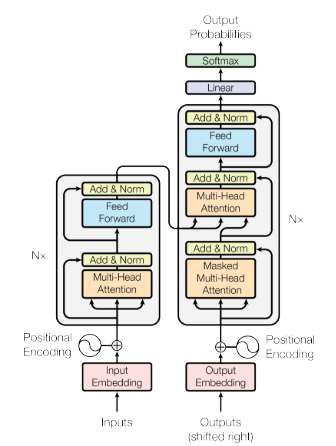
\includegraphics[width=0.6\textwidth]{obrazky-figures/transformers-architecture.png}
    \caption{Architecture of the simulator}
\end{figure}

The standard transformer architecture can be seen at \ref{architecture}, which is the original diagram from the original paper \cite{attention}. To understand why the underlying mechanics of the architecture were the new state of the art for many deep learning tasks, the following subsection will explore the essential parts of transformer architecture in detail. 

\subsection{How Transformers work?}

% todo teorie

This subsection will briefly go through the major processes in a transformer flow. The input sequence of words is first split into predefined sequences of characters called tokens. Tokens can be whole words or only subwords of the original words. Tokenization of sequence is usually done by a tokenizer that can be implemented in specific, more or less complicated ways.

After the tokenization process, the tokens are converted to multi-dimensional vectors using embedding tables or different methods to calculate embeddings for tokens. Embedding dimensions represent different features of the tokens, which are given based on trained parameters. Embeddings are a powerful way how to represent words and are used for different NLP tasks outside of transformers and LLMs, for example, for storing text in vector databases. 

Transformer models can also utilize so-called positional encoding for tokens, which also takes their order into account when calculating the embeddings. This can help identify the right context for specific words because the classical embeddings do not consider that. Positional encodings are generated through the encoding function or can also be done using learned positional encodings.

Furthermore, transformer models and other NLP algorithms and structures might use the softmax function. Softmax function is crucial for obtaining results from calculating weights between different embeddings. For example, it calculates probabilities that match the standard distribution for the output of the decoder of transformer models that are used for determining the probability for the next word of a sequence. The softmax function is not only used for the final result of the transformer process but is also used to normalize the functions when they are being inputted to the next component, as seen in the diagram as \verb|Add & Norm| in Figure \ref{architecture}. 

The main component of the whole transformer architecture is the Attention mechanism. Transformers introduce three different types of attention. Standard attention can be calculated using the following formula from the original paper.

$$Attention(Q, K, V ) = softmax(\frac{QK^T}{\sqrt{d_k}})V$$

Attention allows the vectors in the embeddings to communicate with each other and update their values to better express the context of the whole sequence. The mechanism is a sum of vectors representing Query, Keys, and their respective Values. The scaled Dot-Product Attention is a product of Values with a result of SoftMax normalization of the dot product of Query and Key. The query is essentially the values that the specific vector is searching for in the other parts of the sequence. The key represents the current value of the vector, and the Value is a vector that represents the weight is the current token

Attention can be calculated upon each token simultaneously, so this architecture can be parallelized. The Transformer architecture in the paper used multi-headed attention, attention computed on multiple layers. The layers are concatenated into a single linear output. Attention can help identify connections between tokens in a sequence, so models based on transformer architecture can be much more powerful in tasks such as translation or text generation. Models used for translation usually use Encoder-Decoder attention to track connections between the input and the output to maintain the semantics of the translated sequence.

The original paper's authors also introduced masked attention, which is used by the decoder. It works the same way as standard attention, but it masks the values of tokens that are yet to be predicted, so the model cannot know the exact value of the predicted token.


Transformer architecture revolutionized the field of Deep Learning. Transformers outperformed traditional models like RNNs in translation and text generation tasks thanks to the attention mechanism. The second greatest feature of Transformers was the scalability. The result makes this architecture state of the art to this day, pushing the ability of deep learning models beyond boundaries.
\cite{attention}

% citations: https://blogs.nvidia.com/blog/what-is-a-transformer-model/?source=post_page-----0209f5de0331--------------------------------
% .

\subsection{History of Transformer models}

The number of new deep-learning models based on Transformer architecture has skyrocketed since 2017 \cite{amatriain2023transformer}. This subsection will discuss examples of models that have been significant in the recent history of Transformer models. The variety of Transformer models is currently greater than ever. It is problematic to compare certain models as they have different purposes and functions. The section will mention and briefly explain each significant model to provide perspective into the history and recent development of Transformer models. The timeline of transformer models can be seen in figure \ref{timeline} \cite{amatriain2023transformer}.

\begin{figure}[ht]
    \centering
    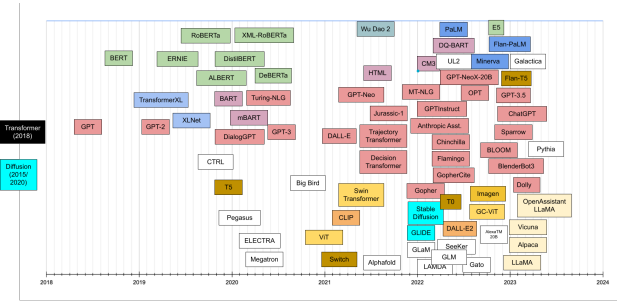
\includegraphics[width=1\textwidth]{obrazky-figures/llm-history.png}
    \caption{Timeline of the Transformer models.}
    \label{timeline}
\end{figure}


\subsubsection{GPT}

The GPT model was the first model that came out after introducing transformers. It was trained on a corpus of 7000 unpublished books \cite{yenduri2023generative}. This dataset helped GPT perform tasks such as answering questions and generating text. The model was trained by an unsupervised learning method and by supervised learning for fine-tuning. This model is a Decoder only, which means it was pre-trained for the next token prediction. This model produced reasonable responses to some extent, but it often hallucinated. Hallucination in terms of the LLM model is when the model outputs nonsensical or not factually correct output. It happens when LLM now has constraints that limit what kind of output it should have or when the prompt or input is ambiguous. However, there might be different reasons, such as lack of training or context misinterpretation. 

\subsubsection{BERT}

BERT stands for Bidirectional Encoder Representation from Transformers. The model was pre-trained with the masked language model (MLM), which enables the attention mechanism to follow both directions. For example, the GPT model was pre-trained in a left-to-right direction. It is an encoder-only model that can perform some specific task. BERT researchers made the approach of pre-training and fine-tuning the model on NLP tasks famous. This approach was then used for different models, leading to the domination of Transformer models in the NLP leaderboards. BERT itself cannot output anything, but thanks to fine-tuning, which consists of adding one layer and retraining the model. \cite{devlin2019bert}


\subsubsection{GPT-2}

The GPT-2 model, with 48 decoders and 1.5 billion parameters, was bigger than its predecessors \cite{Radford2019LanguageMA}. The model is decoder-only, and it does token prediction as GPT-1. It was trained on a corpus of web pages consisting of 500B tokens [2]. It was developed by OpenAI. The main improvement compared to the GPT models was the context window size. It increased from 512 to 1024. The model was able to perform well in a variety of different tasks. 

\subsubsection{RoBERTa}

RoBERTa model is an optimized BERT model with better results. Researchers found that the BERT model was undertrained. Their proposed model achieved, at that time, the best results on GLUE, RACE, and SQuAD benchmarks \cite{liu2019roberta}. These benchmarks test LLMs in several NLP tasks. The main reason for this improvement was the different approach to learning the model. The training relies on randomly masking and predicting tokens. Instead of masking the tokens in ten different ways, the new model uses dynamic masking, greatly improving overall performance. Dynamic masking generates new masks for every sequence injected into the model. 


\subsubsection{GPT-3}

GPT-3 model was a great improvement for the LLM world. The main difference between GPT-2 and GPT-3 is the number of parameters. GPT-3, with over 175 billion parameters, beat all its predecessors \cite{gpt3}. It was trained on five different corpora, including books, crawled websites, Wikipedia, web text, etc. It has better accuracy for the next word prediction. The model's strengths include sentiment analysis, semantic search, code generation, and overall user experience. 

% - few-show, one-shot, and zero shot setting

\subsubsection{LLaMA and open source models}

LLama base model was developed and released by Meta \cite{touvron2023llama}. LLaMA was the answer for OpenAI's GPT models. Meta presented it as a commitment to open science: "As part of Meta’s commitment to open science, today we are publicly releasing LLaMA (Large Language Model Meta AI), a state-of-the-art foundational large language model designed to help researchers advance their work in this subfield of AI" \cite{llamablog}. The model was released in February 2023. However, unlike other LLM models, LLaMA was released as the first model anyone could sign for and download locally. The model was accessible through a Google form \cite{form_2019}; however, the model was leaked on Torrent in March 2023 \cite{andrew_2023}. The LLaMA model and their fine-tuned versions are now available on Hugging Face \cite{llama_2014}. The LLaMA 13B parameter version outperforms GPT-3 (175B) on most of the benchmarks \cite{touvron2023llama}. LLaMA started a new page of LLM models with its OpenSource nature. Researchers and interested developers developed and optimized the models to increase performance and add new features by fine-tuning them. These models compete with the proprietary models from Google and OpenAI. The goal of meta-researchers was to provide the models to the public to explore the safety of LLM technology further. In February of 2023, there were a lot of questions about the state of security of LLMs and the potential impacts. LLaMA was not only a competitor to the other models, but it was also a response to the development of the models.

% todo citace
% https://huggingface.co/papers/2302.13971 [1]
% https://agi-sphere.com/llama-models/ [2]
% https://ai.meta.com/blog/large-language-model-llama-meta-ai/ [3]
% https://arxiv.org/pdf/2302.13971.pdf [4]
% https://docs.google.com/forms/d/e/1FAIpQLSfqNECQnMkycAp2jP4Z9TFX0cGR4uf7b_fBxjY_OjhJILlKGA/viewform [5]
% https://docs.google.com/forms/d/e/1FAIpQLSfqNECQnMkycAp2jP4Z9TFX0cGR4uf7b_fBxjY_OjhJILlKGA/viewform [6]


\subsubsection{GPT-3.5}

% https://openai.com/research/instruction-following

GPT-3.5 was the model that popularized the LLM world. With the release of ChatGPT, everybody with access to the internet could potentially use and experiment with the largest LLM model in the world. \cite{ye2023comprehensive} The main improvement from the older models was the use of Reinforcement learning from human feedback (RLHF) \cite{illustrating}. The model's training consisted of pretraining, creating a reward model to increase success over training time, and fine-tuning the process with RLHF.

%https://arxiv.org/ftp/arxiv/papers/2303/2303.10420.pdf

% https://huggingface.co/blog/rlhf [1]

% https://arxiv.org/pdf/1910.13461.pdf

% https://arxiv.org/pdf/2307.06435.pdf

% citations: https://sanchman21.medium.com/evolution-of-transformers-part-1-faac3f19d780

% https://sanchman21.medium.com/evolution-of-transformers-part-2-f1b94f67abe8

% https://www.analyticsvidhya.com/blog/2023/06/language-models/

% https://sebastianraschka.com/blog/2023/llm-reading-list.html

\subsubsection{Mistral 7B}

Mistral 7B is a 7 billion parameter model trained for performance for multiple kinds of tasks, including commonsense reasoning, word knowledge, reading comprehension, math, code, and other benchmarks \cite{jiang2023mistral}. The results made the model compete with LLamMA models on various benchmarks. Similarly to the LLaMA model, Mistral 7B is an open-source model that allows the community to quantize the model to use less data in cost of performance to fit the model into smaller and more accessible graphic cards, which allows to fine-tune the model with lower costs and also to run it locally. The team behind Mistral also released a fine-tuned version capable of generating text for chat called Mistral 7B instruct. The mistral model utilizes sliding window attention, which allows the handling of longer sequences at lower cost and at higher speed, which can allow potential usage of mistral for real-time applications. The example of mistral shows how the evolution of models makes the models less expensive to run and more accessible for fine-tuning and integrating into different kinds of systems and applications. 


\section{Large Language Models overview}

Large Language models have proven their capabilities for NLP tasks and beyond. This section will provide a broader view of this type of model. The rapid growth of development and advancements of LLM brings new capabilities and opportunities for more sophisticated applications of models in software applications for different systems that require complex problem-solving and human-like interaction \cite{naveed2023comprehensive}. However, it is also important to accurately highlight this new technology's limitations and security concerns. Consequently, a comprehensive understanding of their strengths and weaknesses is essential for creating secure and robust applications. 

Despite the success and strength of LLM models for dealing with certain problems. LLMs have certain limitations. However, it is important to note that with the rapid development of this technology, many of these issues and limitations might be solved or mitigated. 


The main limitation is the computational \cite{naveed2023comprehensive}. Because LLM models require a lot of GPUs to be trained, the training process is expensive. For example, training of the GPT.3-5 cost based on OpenAI's statement above 100 million dollars [2]. This cost can be paid only by the biggest companies in the world, which makes the LLM technology valuable. This was also the reason for the democratization of the LLaMA model. 


Due to the training of LLM on human-generated data, the LLM model can inherit societal biases, potentially leading to ethical concerns \cite{naveed2023comprehensive}. This significant limitation can be partially mitigated through the fine-tuning process. This process can improve the overall safety of the responses. However, it presumes the absence of bias among the individuals involved in the fine-tuning process. Therefore, the mitigation strategy, while beneficial, cannot be foolproof and requires careful implementation and consideration to minimize the potential bias in LLM models.


In specific instances, LLMs demonstrate a phenomenon referred to as "hallucinations" \cite{naveed2023comprehensive}. This term defines scenarios where the responses generated by the LLms are semantically incorrect with the context of the query, exhibit self-contradictions, or deviate from established world knowledge \cite{naveed2023comprehensive}. Such behaviour can be attributed to several factors, including inadequate fine-tuning in certain domains, the presence of ambiguous prompts, or prompts including information outside of the model's training corpus. This limitation is the critical area of focus in the development and refinement of LLMs and is usually improved by human feedback. 

% ethical considerations
The rapid rise and usage of LLM models create questions about ethical considerations concerning these models. The generated content can contain harmful content or content that can be used negatively \cite{naveed2023comprehensive}. This calls for ethical frameworks and policies to govern the outputs of the models. 

% limited knowledge
Information acquired by the LLM during training is limited and can become obsolete after some time. It is expensive to retrain the model frequently. \cite{naveed2023comprehensive} Therefore, models without the ability to search on the web can have limitations of limited knowledge they can provide in their prompts. 


Another limit LLMs have is the limited context window they can provide. Because of that, LLMs tend to forget certain facts after several prompts because they go beyond their context. There are certain breakthroughs like StreamingLLM \cite{xiao2023efficient}. However, most of the current models have a limited context window. Even with the endless context window, there is still a problem with keeping track of the most important facts and information. Another approach for up-to-date knowledge is to use retrieval augmentation generation (RAG). RAG is a method that combines model generation with information retrieval, which enables the model to access external up-to-date knowledge \cite{rag}.

% https://arxiv.org/abs/2309.17453 [2]
% https://www.promptingguide.ai/techniques/rag [3]

Using LLMs comes with a certain risk of generating harmful, misleading or inappropriate content by accident or by giving specific prompts. This behaviour can be replicated using so-called "jailbreak" prompts to trick the LLM into not following safety guidelines \cite{jailbreaking}. Furthermore, LLM can be tricked by "prompt injection" \cite{keary_2023}. Newer LLM models can scrape websites to gather factual information, and this process can accidentally trigger an action given in the scraped website. Therefore, LLM might accidentally leak data or save private user data based on some action given on the attacker's website. 

% todo citace
% https://www.lakera.ai/blog/jailbreaking-large-language-models-guide [1]
% https://www.techopedia.com/definition/prompt-injection-attack

% https://arxiv.org/pdf/2307.06435.pdf
% https://www.wired.com/story/openai-ceo-sam-altman-the-age-of-giant-ai-models-is-already-over/

% https://arxiv.org/pdf/2309.10254.pdf
% https://arxiv.org/pdf/2306.05499.pdf
% https://www.preprints.org/manuscript/202305.0195/v1
% https://www.ml6.eu/blogpost/navigating-ethical-considerations-developing-and-deploying-large-language-models-llms-responsibly

% \section{simulating humans with Large Language models}

% % https://papers.ssrn.com/sol3/papers.cfm?abstract_id=4650172
% % https://arxiv.org/pdf/2310.06500.pdf


\section{Web Interaction Technologies and LLM Integration}
\label{tech}

Nowadays, there are a lot of technologies surrounding the world of large language models. Since the boom of ChatGPT, many developers and companies have tried to use LLms to their advantage. Multiple frameworks enable the integration of LLMs into applications. Technologies such as Semantic Kernel or Lang Chain enable developers to harvest the power of LLMs and use them to analyze data or do difficult tasks in their apps. Moreover, the technology used for web testing and creating apps that interact with the web is crucial for the simulator. Both of the technologies used for LLM integration and web interaction will be discussed in this section. 

\subsection{Web Automation and Interaction}

In web development, web automation tools are essential for web testing. These tools allow control of the website using WebDriver \cite{webdriver_2018}, which created a remote interface for controlling a virtual web browser with instructions. Selenium and Puppeteer, two major web interaction libraries, will be discussed. To create a simulator integrating LLM models, it is crucial to use a library that can aid with such integration, Lang chain \cite{langchain_2023} and Semantic Kernel \cite{semantickernel}. To create an effective simulator capable of mimicking human web browsing, it is essential to leverage capabilities from both web driver libraries that can control the web and libraries responsible for integrating LLMs into software applications. 

\subsubsection{DOM}

Document Object Model (DOM) \cite{dom} is an API for HTML and XML documents. DOM can represent these documents and portray their parts as individual objects. DOM allows interaction and modifications to the documents and access to individual objects. The objects in the DOM have a logical structure similar to a tree-like structure. However, the implementation of the DOM does not specify a tree-like structure.  

DOM is essential for WebDrivers \cite{webdriver_2018} as it allows interaction with the web through a computer program. This is essential for creating a web-based simulator. 

\subsubsection{Selenium}

Selenium is an ecosystem that allows interaction with a virtual web using browser drivers with support for several different browsers, such as GeckoDriver \cite{geckodriver} for Mozilla Firefox, Google Chrome driver \cite{chromedriver} for Chrome browser, etc. The WebDriver is a component that can drive the browser natively or on a remote server. Selenium can be used for viewing the contents of a webpage, initiating actions such as clicks on buttons and references, and inserting text into forms, as well as advanced features like managing cookies together with navigations as a human agent with a browser could. Selenium also supports multiple programming languages like Python, JavaScript, Java, and Csharp. \cite{selenium_2023} 

Selenium allows a fairly straightforward approach to creating web testing scripts. However, it can also be used as a simulator to initiate different actions as a human agent would. This includes dynamic elements such as pop-ups and advanced web page structures. The main advantages of the Selenium environment are its open-source nature, multi-language support, and the variety of interactions it can perform.

\subsubsection{Puppeteer}

Puppeteer cite{puppeteer24} is a library providing an API for Chrome over the Dev Tools protocol \cite{devtools}. Puppeteer was made to test the performance and functionality of web pages or for web automation. It can perform interactions users could do manually. The library can also work with single-page and Server-side rendering web applications. Puppeteer is officially developed for JavaScript language. However, some unofficial libraries support Puppeteer usage within different languages, such as Python. \

Compared to Selenium, Puppeteer brings a functional alternative that can outperform selenium in certain cases as it focuses mainly on chromium drivers. However, the only official language support can be a disadvantage when creating a simulator that has to be robust, especially when JavaScript language is not suitable for such use cases. Puppeteer could be used for specific scenarios where Selenium cannot perform a given task. 

\subsection{Large Language Model Integration}

LLMs can dramatically influence the way applications are structured and developed. With the ability to integrate LLMs into software applications, developers can use LLMs to perform complicated tasks that are hard for algorithmic approaches and can solve the ambiguity of certain use cases. Semantic Kernel \cite{semantickernel} and Langchain \cite{langchain_2023} are the two main ecosystems used for this process. Both have different integration approaches and allow different solutions. Both Langchain and Semantic Kernel will be discussed. 

\subsubsection{Semantic Kernel}

Semantic Kernel \cite{semantickernel} is an open-source SDK designed to integrate AI with software applications. It can integrate models from platforms like OpenAI, Azure OpenAI or Hugging Face. This SDK can be used in Csharp, Python and Java applications. Semantic Kernel allows for creating AI agents that can take on various tasks. The tasks include answering questions or automating different processes. The main feature of Semantic Kernel is the orchestration layer, which allows for seamless connection of AI models and plugins that add extensions for existing LLM models, such as the math plugin that allows the LLM model to calculate expressions to get accurate results. 

\subsubsection{LangChain}

Langchain \cite{langchain_2023} is a Python library designed for building applications that leverage LLM models like GPT-3. It provides a framework for combining different components of LLM models in a modular and flexible way. Langchain uses LangChain Expression Language (LCEL), which is short for creating pipelines called "chains" with certain logic. 

One of the key features of LangChain is the ability to create agent applications or applications where an LLM model is used for reasoning. LangChain also implements the ReAct \cite{yao2023react} method to help the model reason and solve problems using the available tools. 

LangChain can be particularly useful in simulating human behaviour in browsers. It can help create systems that mimic human browsing patterns by making decisions based on current webpage information given to the LLM model. This can include clicking on buttons, filling in search and input forms, understanding the text, and taking actions based on the current context. 

%todo - chains and prompt templates and their flow

% chat prompts and chatbots

% output parser

%todo - document loaders 

%todo - advantages


%  https://www.langchain.com/ [1]
% https://python.langchain.com/docs/get_started/introduction

% existing simulator
% input to the simulator?j
\
% architecture
% components
% scope 
% high-level functionality
% 

\chapter{Design and Architecture}
\label{da}

This chapter will investigate the components and scope crucial for a functional and robust simulator architecture that replicates human behavior with the power of LLM. The objective is to create a simulator that enables replicating human behavior in web browsing.

\section{Objectives and Components}

There are several objectives for the simulator. The most important is the accuracy of navigation through a website compared with human behavior. The main objective of the simulator is to perform actions based on a given goal. The goal is a text representing what will be accomplished in the simulation. Because the simulator will not necessarily have prior information about the website and its structure, each page throughout the simulation has to be processed individually. The main component of the simulator is the decision-making model that decides the next interaction on the website. The input to the simulator is a specification of a goal and a URL to an existing website, together with additional parameters influencing the simulation behavior that is later described in the section \ref{conf}. The simulator outputs are the logs representing the navigation path throughout the simulation, the actions done on the website, and information about requests made between the browser and the website. Logging and what data is stored is specified in a later section \ref{logging}. The simulation ends when the decision goal of the simulation has been achieved.

 % To truly simulate human behavior, the simulator will not necessarily have prior information about the website it will visit. It will have to do everything on its own. The model will have prior information about a type of character it should simulate and its past actions. Another important part of the simulation is the outcome. In this case, the simulator will produce logs from the website and also from the actions it will perform together with other information about the process of the simulation. These logs can be used for comparison with human actors, but they can also be used as a training dataset. To make the simulator more usable in real use cases, it has to be parametrized. There will be an emphasis on parametrization to allow users to customize the behavior of the model through certain parameters and also influence certain characteristics of the simulator. Furthermore, the aim is to create an accurate simulator for human web browsing that can navigate and complete certain goals without any prior information about the website. An LLM will construct the goals that must be completed on the website. It can have certain restrictions, but it should behave on its own as much as possible.

\section{Architecture}

This section introduces the key components of the simulator and how they work together. Furthermore, it explains the high-level flow of the application during a simulation. The simulator is composed of three main components:

\begin{itemize}
    \item Virtual Web Browser,
    \item Web Controller,
    \item Decision Making Model,
\end{itemize}

% The architecture of the simulator has components that have been discussed in the previous section.  Each of the components will be discussed individually in each subsection. Components of the simulator therefore are Web Browser, Web Controller, and Decision Model.

\begin{figure}[H]
\label{arch}
    \centering
    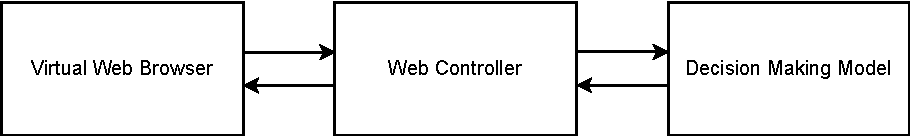
\includegraphics[width=1\textwidth]{obrazky-figures/architecture_small.pdf}
    \caption{Architecture of the simulator}
\end{figure}

The simulation flow is visible in Figure \ref{arch}. Firstly, the Web Controller gets the key information, the URL of the website, and the goal that should be accomplished. It sends a command to the Virtual Web Browser to load the website of a given URL and then sends the raw data of the website back to the Web Controller. Then, the Web Controller parses the raw data from the website into a structured form containing links and contents and passes it to the Decision Making Model. The Decision Making Model returns the most relevant interaction to the Web Controller, passing it to the Virtual Web Browser that updates the page. This loop repeats until the goal is achieved, then the simulation terminates. 


% During the simulation, the flow of interactions is as follows. Firstly, based on configuration, the simulator gets the URL of a webpage and the goal that should be accomplished. The Web Controller loads the website and extracts information from the current page using the Web Parser as seen in figure \ref{arch}. The extracted information is then parsed by a Parser that extracts data used in an input prompt to the Decision Maker component. Furthermore, the Decision Maker component has its own logic that takes input from the parsed web information, its own memory component and information from Web Controller of the available actions. The Decision Maker then makes a decision and chooses next action that is propagated to the web controller which invokes it. Lastly, the state of the webpage is changed  by the chosen action and whole process starts over. The simulation ends when the Decision Model concludes that the initial goal is completed and chooses special actions that initiates the end of simulation.

\subsection{Virtual Web Browser}
\label{vbc}

The Virtual Web Browser has two main functionalities. Firstly, to download and display the content of a given web page, which is then passed in a raw format to the Web Controller. Secondly, to execute commands representing users' behaviors on the website, such as:
\begin{itemize}
    \item input to a search bar,
    \item click on a button,
    \item click on a link.
\end{itemize}

\subsection{Web Controller}

The Web Controller is the middle layer between the Decision Making Model and Virtual Web Browser. It has four main functionalities:

\begin{itemize}
    \item gets web data from the Virtual Web Browser,
    \item parses the data and sends it to the Decision Making Model,
    \item receives a selected interaction from the Decision Making model,
    \item sends the interaction to the Virtual Web Browser in the correct format.
\end{itemize}

The information obtained from the Virtual Web Browser is in HTML format and has to be parsed. The Web Controller contains a web parser that allows the raw HTML to be parsed in a structured format. The interactions received from a Decision Making Model have to be parsed again from a general format to a format that the Virtual Web Browser understands. 


\subsection{Decision Making Model}
\label{dmm}

The Decision Making Model is the core part of the simulator. It receives information from the current page in a structured format, selects the most optimal interaction, and propagates it to the Virtual Web Browser with the help of the Web Controller. To make better predictions, the Decision Making Model uses internal memory of past actions.

\subsubsection{Interactions}

The interactions are modeling human behavior that is simulated in the simulator. The decisions a human agent would make while browsing are abstracted into a fixed list of four types of actions. The actions were selected to enable the most common interactions with a website. The types of actions are:

\begin{enumerate}
    \item click on a link or button,
    \item use a search bar,
    \item retrieve information from the current page,
    \item exit the simulation.
\end{enumerate}

Action that handles clicks on a website was created to enable navigation on the website during the simulation. The action to use a search bar is there because most current websites have a search bar, which enables fast navigation and searching for detailed information. 

Even though the last two actions are not part of the physical actions a human would make on a website, they are crucial for the simulator. Information retrieval is used mainly to allow the Decision Model more context because the standard content of the webpage obtained from the Web Controller might be limited. The exit action is used for the Decision Making Model to exit the simulation upon the goal being accomplished.

\subsubsection{Output Format}

The Decision Making Model is powered by the LLMs. To make the LLMs understand the context and create better outputs, the following output has a given form of three attributes:

\begin{enumerate}
    \item Thought,
    \item Action,
    \item Action Context.
\end{enumerate}

% thought helps to show reason of LLM

Each of these attributes has special functionality. The Thought component represents the reason for a specified action. It was created to help the LLM structure the output with an initial piece of information that adds context to the decision and reason for the decision.

Secondly, the Action holds the name of the action selected from the list of actions. It only contains information about the action type.

Lastly, The Action Context serves as additional information used by the Web Controller. For example, to click on a given link, the Web Controller must receive the link's name; this name must be contained in the Action Context. 

The given format of the output that the Decision Making Model is used to reduce hallucinations made by the LLMs and create an abstraction of human behavior. 

%The LLM model will be a core part of this process. It will be given a prompt with a predefined structure with variable data based on the current view of the page. It will also receive information about the history of its choices. It will choose the best following action to be performed. This will trigger the webcontroller to perform such action and rerender the view of the webpage. The new view will be scraped and parsed, processed by the web controller and also given to the LLM to perform the following action. The LLM model will also have to decide if the initial goals have been fulfilled.

%The goal is to decide on the LLM model as easily as possible, and ideally, it should be the correct one on the first try. To increase the success rate, there will be cross-checking mechanisms designed to correct the decision if needed. 

% - solution for a particular problem

% - defines the scope of the model
\section{Scope}

The simulator proposed in this thesis is designed to simulate human behavior on a website. The extent to which the simulator can represent human behavior is given by the architecture and the list of actions that are defined in subsection \ref{dmm}. The scope of the simulation defined the goals and websites that could be used for the simulation. The website must not contain a CAPTCHA challenge or other human verification methods. Secondly, the website must be functional without malicious content that could negatively influence the simulation. The goal specification must be clear and accomplishable on a given website. The architecture does not model real-time decision-making. Therefore, the timing of the action is not influenced by the real frequency of human decisions but rather by configurable timeouts discussed in section \ref{conf}. The fixed list of actions defined in subsection \ref{dmm} defines what goals can be accomplished by the simulator.

In summary, both the design and implementation are tailored to specific use cases, including web navigation and the extraction of facts and information from websites, where the extraction of facts is mainly on granting the simulator information needed for determining the goal completion.

\chapter{Implementation}
\label{imp}

This chapter explores and explains the simulator implementation defined by the design architecture explained in chapter \ref{da}. The simulator is created as a~command-line interface application. It is implemented in Python with the two main libraries, Langchain and Selenium. 

Firstly, the Selenium library is used for a Selenium driver that creates a headless browser that implements the Virtual Browser Component \ref{vbc}, and it can handle the interactions while receiving updated information from the browser. 

Secondly, The Langchain library integrates LLMs and the program itself. Langchain handles the proper format of actions sent to Selenium and provides means for creating an interface that handles the core decision-making throughout the simulation. Furthermore, the implementation contains supporting components that handle configuration, the application's core, logging mechanisms, and parsers of the data obtained from the webpage or the LLM. 

The implementation is logically separated into parts to improve maintainability and add features in future work. Each component of the simulator will be described in each section with information about it to understand the communication of other parts of the architecture.

% diagram of the architecture and overview of the implementation

\section{Configuration}
\label{conf}

Configuration in any application enables a simple and fast way how to change the behavior of the applications for different use cases that increase flexibility and also maintainability. In this case, the configuration is implemented by a simple JSON parser component that propagates the values to the application. The JSON configuration is defined by the following JSON schema \footnote{JSON schema converted available at: https://transform.tools/json-to-json-schema}:

\begin{verbatim}
{
  "$schema": "http://json-schema.org/draft-07/schema#",
  "title": "Generated schema for Root",
  "type": "object",
  "properties": {
    "website": {
      "type": "string"},
    "goal": {
      "type": "string"},
    "request_rate": {
      "type": "number"},
    "persona": {
      "type": "string"},
    "llm_provider": {
      "type": "string"},
    "model_name": {
      "type": "string"},
    "temperature": {
      "type": "number"},
    "verbose": {
      "type": "boolean"},
    "initial_timout": {
      "type": "number"},
    "timeout_per_action": {
      "type": "number"},
    "web_data": { "type": "object",
      "properties": {
        "type": {"type": "string"},
        "name": {"type": "string"}},
      "required": ["type","name"]},
    "cookie_config": {
      "type": "object",
      "properties": {
        "buttons": {
          "type": "array",
          "items": {
            "type": "object",
            "properties": {
              "type": {
                "type": "string"},
              "name": {
                "type": "string"}},
    "required": ["type","name"]}}},
    "required": ["buttons"]}},
  "required": ["website","goal","request_rate"
  ,"persona","llm_provider","model_name",
  "temperature","initial_timout","timeout_per_action",
  ]
}
\end{verbatim}

An example of a functional configuration is the following JSON file:

\begin{verbatim}
{
    "website": "https://www.python.org/",
    "goal": "Find upcoming events happening in USA",
    "request_rate": 30,
    "persona": "Generic",
    "llm_provider": "openai",
    "model_name": "gpt-4-turbo",
    "temperature": 0.45,
    "verbose": true,
    "initial_timout": 3,
    "timeout_per_action": 0,
    "web_data": {
        "type": "class",
        "name": "search-text"
    },
    "cookie_config": {
        "buttons": [
            {
                "type": "id",
                "name": "onetrust-reject-all-handler"
            }
        ]
    }
}
\end{verbatim}

Firstly, the configuration allows the user to specify a website using a URL and goal in plaintext in human-like language, specifying where the simulation will occur. The configuration allows the selection of an LLM provider, as explained in the section \ref{provider}. The model allows selecting a particular LLM model from models accessible throughout the selected LLM provider. The persona option enables the selection of a predefined persona that is defined in the LLM provider \ref{provider}. The user has the option to set timeouts used for a time the application takes between actions or before the simulation used for proper loading of the website before it load its contents. Next, the web data component allows for specifying the information used to access the search bar on websites where the search bar id is not found using the standard web parser. Similarly, the cookie configuration allows the user to resolve the cookie popup that appears on certain websites.

\section{Web parsing}

In each iteration of the main application loop, the LLM needs information from the website to understand the next optimal action for achieving the predetermined goal. The application implements two ways of gathering and preparing data for the LLM to access. 

The web is parsed to collect all available \texttt{<a> href} attributes, buttons, and input fields. The raw data are obtained from the selenium method \verb|get_source| and are parsed and enriched to more information by selenium methods that allow searching for IDs or text for particular elements. In each iteration, the web parser looks for search bar input by looking for an ID with a~substring that contains the keyword \textit{search},\textit{query}, or other familiar keywords, which works for most websites. For websites where the ID for the search bar is different, the user can configure the ID for the element so the decision chain can use the search bar action as discussed in section \ref{conf}. 

The second type of web data is a webpage summary generated for every decision. This summary helps the decision chain understand what type of content is on a given URL. In certain cases, it can help the LLM understand if the desired information it needs to retrieve is present in the current state of the simulation. Lastly, it helps the decision chat to reduce hallucinations where the llm does not know if the webpage's content has changed. 

% todo fix if it changes
\section{LLM Chains}

The application implements two Langchain chains: a decision chain and actions chains made to parse the input for a selected action in a given format. These two chains are in the core part of the program and handle the decision of actions by LLM and subsequent interpretation of the output together with action invocation by the action chains.

\subsection{Decision chain}

The core of the application is the decision chain. It is implemented by a chat prompt and output parser in JSON format. The prompt template introduces the LLM to the simulation of human behavior and instructs it to decide what action should be chosen from a specific list of actions on a website URL address. The LLM is informed about the goal that should be accomplished. With each interaction of the application loop, the chat gets information about the current URL, goal, list of hrefs, website summary, and past actions. The chat then outputs a decision in three components, as shown below.

\begin{verbatim}
    {
    "Thought" : <thought of the llm>,
    "Action" : <action chosen from the list of actions>,
    "Action context" : <the detailed information of the action>,
    }
\end{verbatim}

The thought is used to help the LLM formulate the output, starting with a thought of the action that will be chosen. The action then includes the name of the selected action from the list of actions. The action context includes the data for the action that has been selected.

The available list of actions:

\begin{itemize}
    \item Use a search on a current URL
    \item Retrieve information from current URL
    \item Click on a button or a link
    \item Exit simulation
\end{itemize}

The LLM model can use the list of actions to navigate the website and retrieve information to accomplish a current goal. Each action is then handled by its specific action chain.

The output from the decision chain includes a JSON parser implemented inside the Langchain library. However, as the JSON parser can fail in certain scenarios, it has to be checked with an additional parser that checks the structure based on a~given schema.If the output schema is not met or there is an error with the standard parser. The output from the main chain is given to a chain called \verb|fix chain| that is used for fixing the incorrect structure of the output. When all parsers fail, or there is an error with the invocation of a current action, the LLM is informed about the result in the next iteration throughout the memory component and can react to the situation.

\subsection{Action chains}

When the decision is made by the decision chain, the LLM's output is given to one of the four chains responsible for the subsequent actions. Each chain is specialized for handling a given action. By dividing the task of a decision and action into smaller tasks, a chain reduces hallucinations by giving the LLM less 'work.' 

The chain responsible for clicking on an element outputs the name of the button or link in a given format by an output parser to JSON. This simplifies the parsing of the decision chat because the content or the button's name might not be consistent in the provided output of the decision chain. The parsed output from the action chain is then directly used to call a Selenium driver method to interact with a~given element. 

For the search action, the chain output is a keyword inputted into a search bar on the browsed website. In certain situations, the decision chain outputs a sentence with the content of what it wants to search for, and the search chain selects a~keyword or set of keywords that best defines the searched content. The output is then used again to handle the selenium driver's actions. 

Retrieving data from the website does not need a chain to better structure the output used by selenium, but a different approach handles the process. The action extracts data from a current URL using a web loader method implemented in the long chain library that enables reading data from a website and parsing it only to textual content. LLM retrieves information relevant to the context of the given retrieved action. When the current URL contains a large amount of data, the retrieve action utilizes embeddings of the content that can be generated, and the LLM can query for a chunk relevant for the action context. 

The exit action is not implemented using an LLM chain, so this section does not need to be discussed. 

\section{LLM provider}
\label{provider}

To create a robust and maintainable component for handling a connection to a LLM. The simulator implements a separate component of an LLM provider that is used in the chains. The LLM provider is Factory, which instantiates objects of specific LLM providers defined by a class. Each class of LLM providers must implement the connection to the model and return the chains used in the application. The methods are polymorphic and are called in the main application loop. For different LLM providers, the exact implementation of the chain might differ. The implemented providers in the simulator include OpenAI and Mistral LLM providers. This structure allows for a possible extension of the available providers for other LLM models of all kinds of forms or possibly different models that follow the IO of the whole application schema. The LLM provider also handles different personas configured in the configuration and defines what personas are available for selection. For the purpose of this work, the Generic persona type was used.

\section{Selenium controller}

The selenium driver is initialized at the beginning of the simulation. The application uses a Firefox browser as it has fewer prerequisites for installation. The website is loaded by a method \verb|.get()| method provided by the driver object. 

The interaction with the website consists mainly of finding elements the application wants to interact with by ID, link name, or other attributes. For clickable links or buttons, the selenium driver uses \verb|.click()| method to click the given element; for inputting data into input fields, selenium uses \verb|.send_keys()| with the content that should be inputted.

For handling search bar information, the input element is firstly clear using \verb|.clear()| method, and after the keys are sent, the enter key is used to submit the query.

At the end of the simulation, the driver object is also used to retrieve the requests made between the browser and the website. It contains requests made by and to advertising websites. The requests are stored in a log file. The list of requests can be retrieved using \verb|driver.requests| iterable. 

% todo structure method

\section{Logger}
\label{logging}

The application utilizes logging, a standard Python library, to handle and manage logs throughout the runtime. The implementation uses two different logs. The first log provides information about the states of the application and warnings or errors that might occur during the runtime. This log type is displayed in the terminal and written to a log file \verb|log.txt| where it is stored for a single simulation run. The second logger is used for logging information about the chosen actions and their context stored in a different file \verb|log_actions.txt| and is used for analysis made by the benchmarks /ref{bench}. 

The logs of requests caught during the simulation and obtained by the Selenium driver are parsed in a simple method and saved to a file called \\\verb|simulation_requests.ndjson| with a structure.

\begin{verbatim}
    {"method": <method>,
    "url": <URL>,
    "headers": <headers>,
    "body": <body>,}
\end{verbatim}

optimal for the input for a classification used later in the \ref{experiment} section

The configuration can specify file names and the path of the logs, or optionally. It can turn off the file or standard output options.

\section{Challenges}

The main challenge that had to be tackled is the LLM context window is limited to a certain number of tokens; therefore, the data needs to have certain preprocessing, mainly the web page summary and the data retrieval action. Therefore, the llm is only a portion of the data because the summary or parsing omits a portion humans could perceive. The memory component then has to be limited and only contain a~short portion of data and has a certain length.  

Secondly, the application is limited to the actions it can perform. These actions are used in most human traffic where humans need to get information on the web or navigate a website.

Furthermore, web summary, parsing, and decision-making take several seconds to complete. In a context where the goal is to simulate human behavior, the delays prove advantageous, mirroring the natural pace of human decision-making. 

The work was mainly focused on exploring the ability of the LLM to simulate human behavior in web navigating and data-retrieving tasks. The application could be overhauled for more complex web tasks in future work. 

\chapter{Experiments and Testing}
\label{experiment}

This chapter will discuss the three types of experimentation and tests used to test and grade the application's usability and similarity to human behavior or web traffic. The system testing consisted of three types of tests aimed at different aspects. The application was first tested using automated benchmarks to determine the simulation's success rate and grade its performance together by retrieving valuable metrics rating its performance on a given website and goal. The second experiment compares the simulator and humans using calculated metrics. Lastly, the final experiment compares differences and similarities in web navigation between the simulator and human data. 

\section{Website selection}

Both the human data and data obtained by the simulator contain selected websites with specific and different goals for each website. The websites with their goal are:

\begin{itemize}
    \item Python.org with the goal 'Find information about Python events in the Netherlands,
    \item Dictionary.cambridge.com with the goal 'Find the definition of the word Fungus',
    \item Wikipedia.org with the goal 'Find when Václav Havel completed his secondary education',
    \item u.gg/champions with the goal 'Find counter for champion Ahri',
    \item rottentomatoes.com with the goal 'Find the name of the director who made the film Monty Python and The Holy Grail.
\end{itemize}

The websites were chosen to represent unique website types with different use cases. Each goal can be achieved with a different combination of actions. To successfully complete the goal in a given simulation, the Model has to navigate to a webpage containing the searched information and retrieve the information either using the web summary or by performing the retrieve action. The success rate of different simulation runs was measured using the benchmarks.

\section{Benchmarks}
\label{benchmark}

The benchmarks were implemented in a separate Jupyternotebook to test the simulator and record metrics used for evaluation. They come with the standard simulator configuration with additional parameters, like the number of repetitions of a simulation run. Additionally, benchmarks allow the creation of a list of different simulations with unique configuration settings. The results of the benchmarks are used to calculate metrics used for experiments. 

\subsection{Configuration}

To understand how the benchmark functions. The following example of a benchmark configuration shows its functionality.

\begin{verbatim}
{
    "benchmark_name": "experiment_data",
    "simulations": [
        {
            "provider":"openai",
            "model":"gpt-4-turbo",
            "request_rate":30,
            "verbose": "true",
            "initial_timout": 3,
            "website_name_short" : "python-org",
            "website": "https://www.python.org/",
            "goal": "Find info about Python events in the Netherlands",
            "target_urls": [
                "https://www.python.org/events/python-events/",
                "https://www.python.org/events/"
            ],
            "final_action": "Retrieve",
            "runs": 3
        },
        ... 
    ]}
\end{verbatim}

The benchmark configuration is a list of configurations for the goal, website, and target URL and action. Target URL and action can help determine whether the simulation was successful based on the final URL and action before the action Exit.

\subsection{Output}

The benchmarks are recording several metrics to allow for metric calculation. The metrics are stored in a specific path as a JSON file or logs and raw data. An example of a simulation benchmark:

\begin{verbatim}
    {
    "exit": false,
    "goal_complete": false,
    "action_count": 7,
    "action_per_type": {
        "Search": 1,
        "Click": 6,
        "Exit": 0,
        "Retrieve": 0
    },
    "simulation_length": 78.07544684410095,
    "average_time_per_action": 11.153635263442993,
    "raw_data": [...]
\end{verbatim}

The key \verb|exit| and \verb|goal_complete| is used to determine whether the simulation was successful. The key \verb|action_count| is used for measuring the number of actions. Furthermore, \verb|action_per_type| displays the distribution of actions based on their type. The keys also contain information about the length of the simulation and average time per action in fields \verb|simulation_length| and \verb|average_time_per_action|. The JSON file also contains a list of parsed \verb|actions.txt| log.

The JSON files are stored in a specific path in a directory \verb|experimend_data| with a specific path. The subdirectories contain the model's name specified in the benchmark configuration, e.g., \verb|gpt-4-turbo|. The subdirectory of a model directory contains the name of the \verb|website_name_short| field from the benchmark configuration. Finally, the website directory contains JSON files of each run of one specific benchmark. The JSON files containing the simulation data are created to be unique with a specific pattern of their name: \verb|D_HH_MM_SS_runnumber_metrics.json| to avoid duplications. Example path to a specific JSON file can be as follows:

\begin{verbatim}
\experiment_data\gpt-4-turbo\python-org\05_23_40_32_0_metrics.json
\end{verbatim}

The results from the directories are parsed and aggregated to produce metrics for each model and specific sites. The aggregated metrics include the following:

\begin{itemize}
    \item average number of actions per simulation,
    \item average time for action in simulations,
    \item average length of simulations,
    \item and success rate of simulations.
\end{itemize}

The results are used in a specialized Jupyter notebook to create graph representations of the data to compare the results. The benchmark helps create an automated pipeline for recording and storing data from multiple simulation runs with different metrics and automatically creating graphs.

\section{Human Data collection}

The human data were collected using a Google form \footnote{form available at the link: https://forms.gle/DNrDNpKr7VzPV7h98 with a requirement of a Google account because it requires upload of files to Google Drive}. The form contains instructions and the same set of websites and predefined goals as used for the benchmarks. To effectively collect the user interaction the users used Selenium IDE\footnote{chrome extension: Selenium IDE available at https://chromewebstore.google.com/} chrome extension and screen recording extension\footnote{Screen Recorder, available at: https://chromewebstore.google.com/}

The Selenium IDE extension was used to record user interactions with the website in a JSON-like format. The data from the video recording was used because the Selenium IDE extension does not store timestamps and current URLs of actions. The data was annotated using video recordings.


\section{Experiments}

The experiments compare performance between LLMs GPT 3.5 Turbo and GPT 4 Turbo based on success rate. Furthermore, the experiments show the differences and similarities based on calculated metrics between the simulator and the human data. The last experiment shows differences between web navigation on the five websites using a Sankey diagram.

\subsection{Success rate}

\begin{figure}[H]
    \label{success}
    \centering
    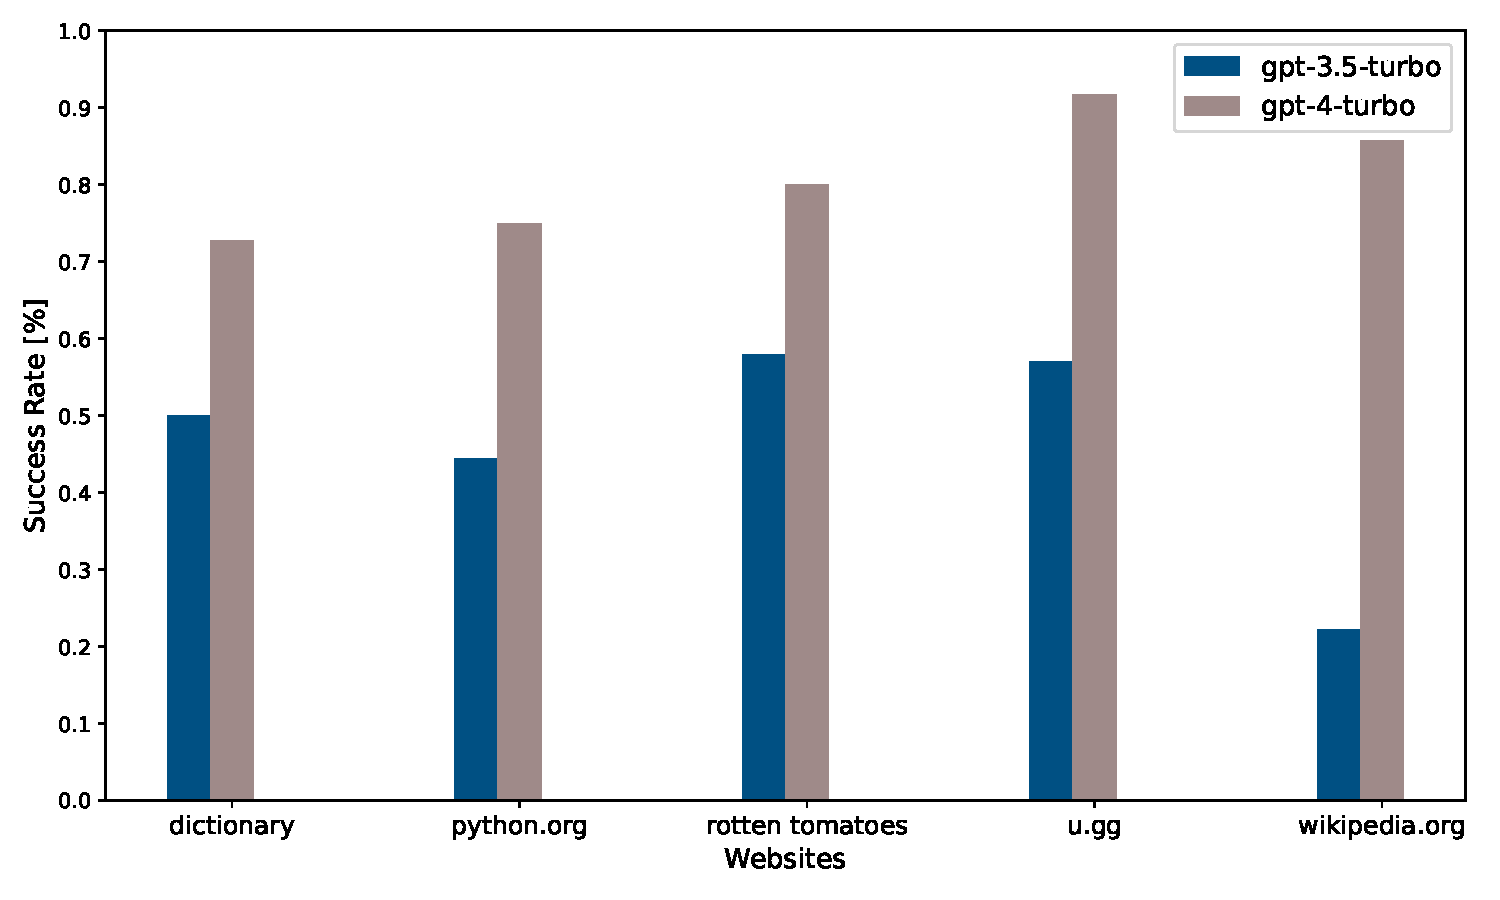
\includegraphics[width=1\textwidth]{obrazky-figures/success_rate.pdf}
    \caption{Success Rate by Website and Model}
\end{figure}

Figure \ref{success} shows the success rate of models GPT 3.5 Turbo and GPT 4 Turbo on the five websites. The plot shows success rates around 50\% for model GPT 3.5 Turbo on four websites and a lower success rate for website Wikipedia.org. On the other hand, GPT 4 Turbo shows an increase in the success rate across all of the websites, averaging on 82.1\% success rate. For the model, GPT 3.5 Turbo, the simulation failed mainly due to the model's hallucination. Meanwhile, GPT 4 Turbo failed in situations caused by a selenium driver or timeouts caused by the website. Finally, the results show the usability of the system and a great improvement in success rate with model GPT 4 Turbo. 


\subsection{Comparison on metrics with human data}

The following experiments show metrics results compared between humans and the simulator with two models, GPT 3.5 Turbo and GPT 4 Turbo. The metrics include:

\begin{itemize}
    \item average simulation time,
    \item average number of actions per simulation,
    \item average time for action,
\end{itemize}

\subsubsection{Simulation time comparison}

\begin{figure}[ht]
    \centering
    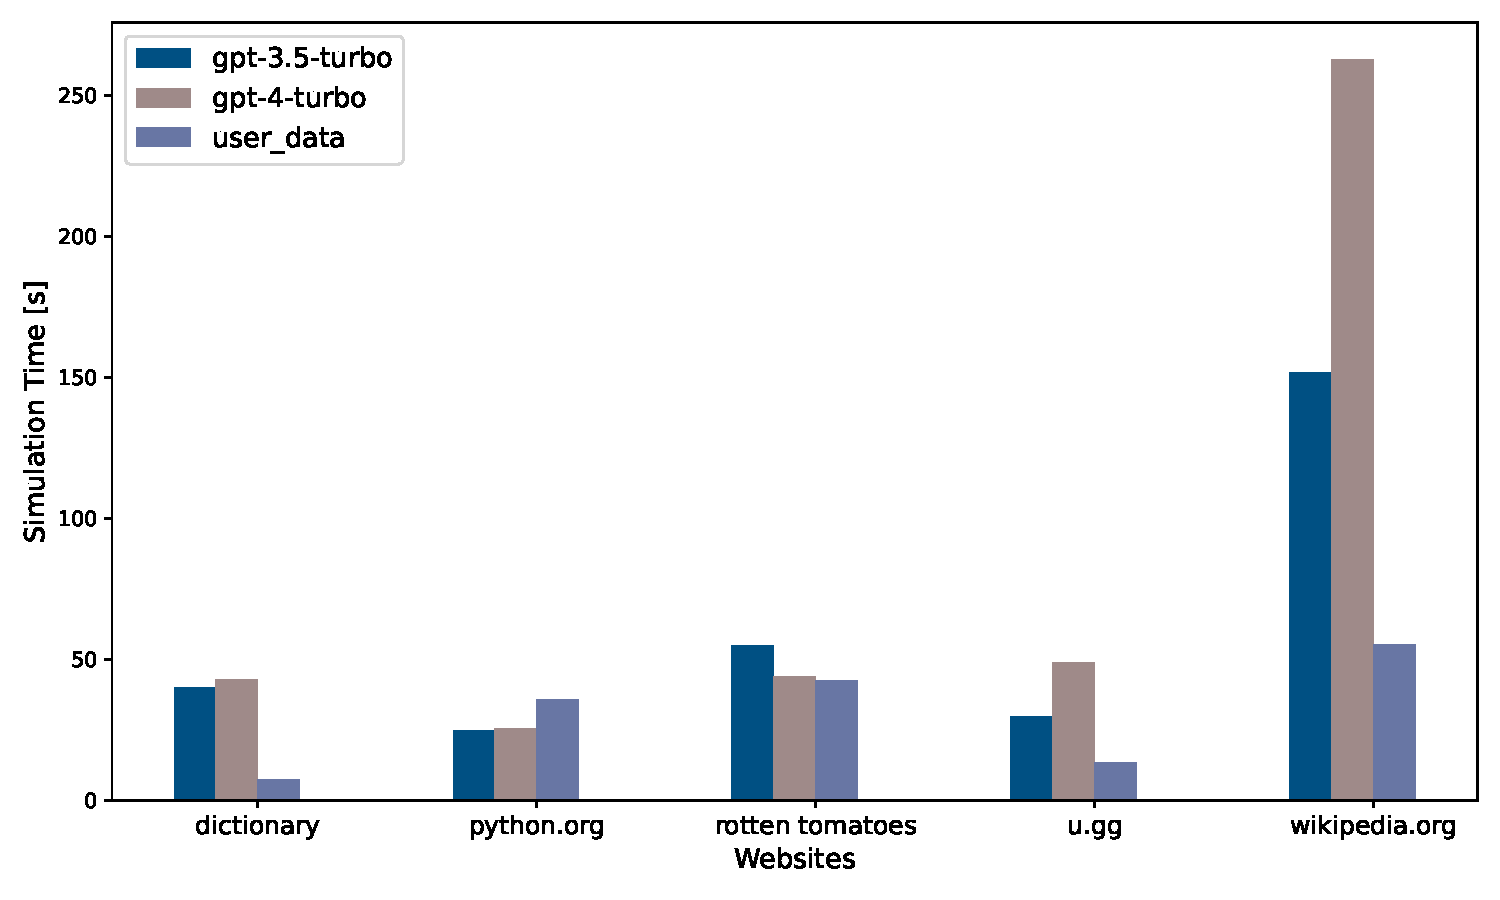
\includegraphics[width=1\textwidth]{obrazky-figures/simulation_time_comparison.pdf}
    \caption{Average Simulation comparing Humans and LLM models}
    \label{time_comp}
\end{figure}

The average simulation time between LLMs and Humans shows different results for each site seen in Figure \ref{time_comp}. On average, humans have shorter simulation time than LLMs. The biggest difference is on the Wikipedia website.

The high difference is caused by the large amount of content on the page that has to be processed by the simulator, which takes a few seconds per LLM query result per simulation loop. The difference between the models and humans is smaller for other websites because they have less content. For the website Python.org, the LLMs have a lower simulation time. This shows one of the differences between the simulator and human data. However, except on the Wikipedia page, the differences are not that dramatic. 

\subsubsection{Action count}

\begin{figure}[ht]
    \centering
    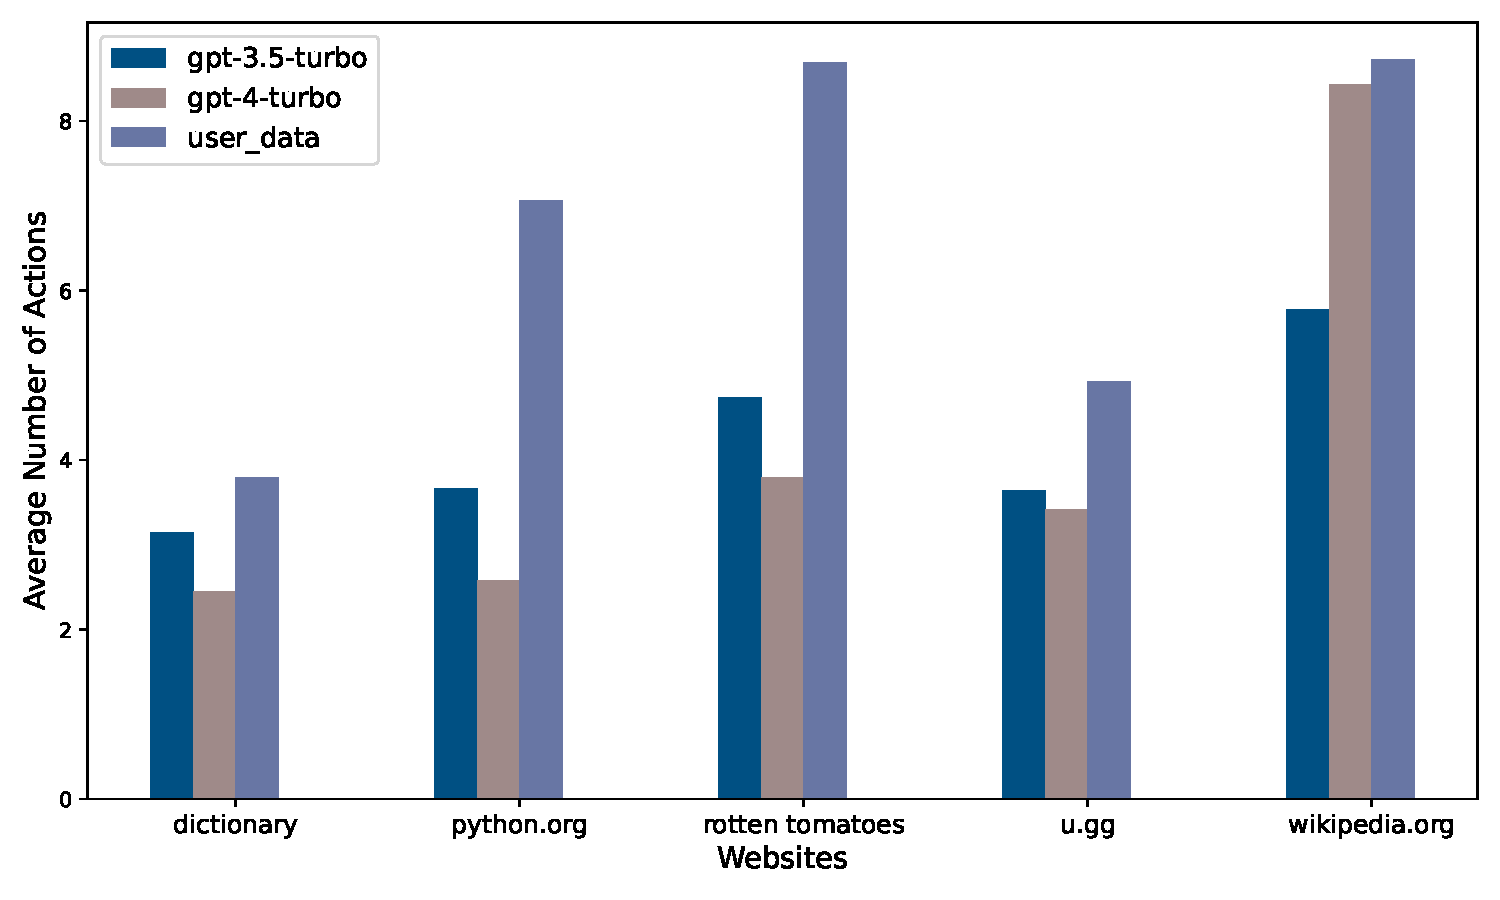
\includegraphics[width=1\textwidth]{obrazky-figures/actions_count_comparison.pdf}
    \caption{Actions per simulation}
    \label{aps_comp}
\end{figure}

Figure \ref{aps_comp} The average count of actions per site shows a high number of actions for the human respondents and a lower number for LLM models. The LLMs during the simulation tend to select accurate results because of the architecture of the simulator that provides detailed information on each webpage, which helps the LLM to make the best actions in a given state. This shows that the average number of actions for LLMs tends to be lower than for humans, showing yet another difference between humans and the simulator. However, the simulator was designed to complete the goals the most effectively.

\subsubsection{Time for action}

\begin{figure}[H]
    \centering
    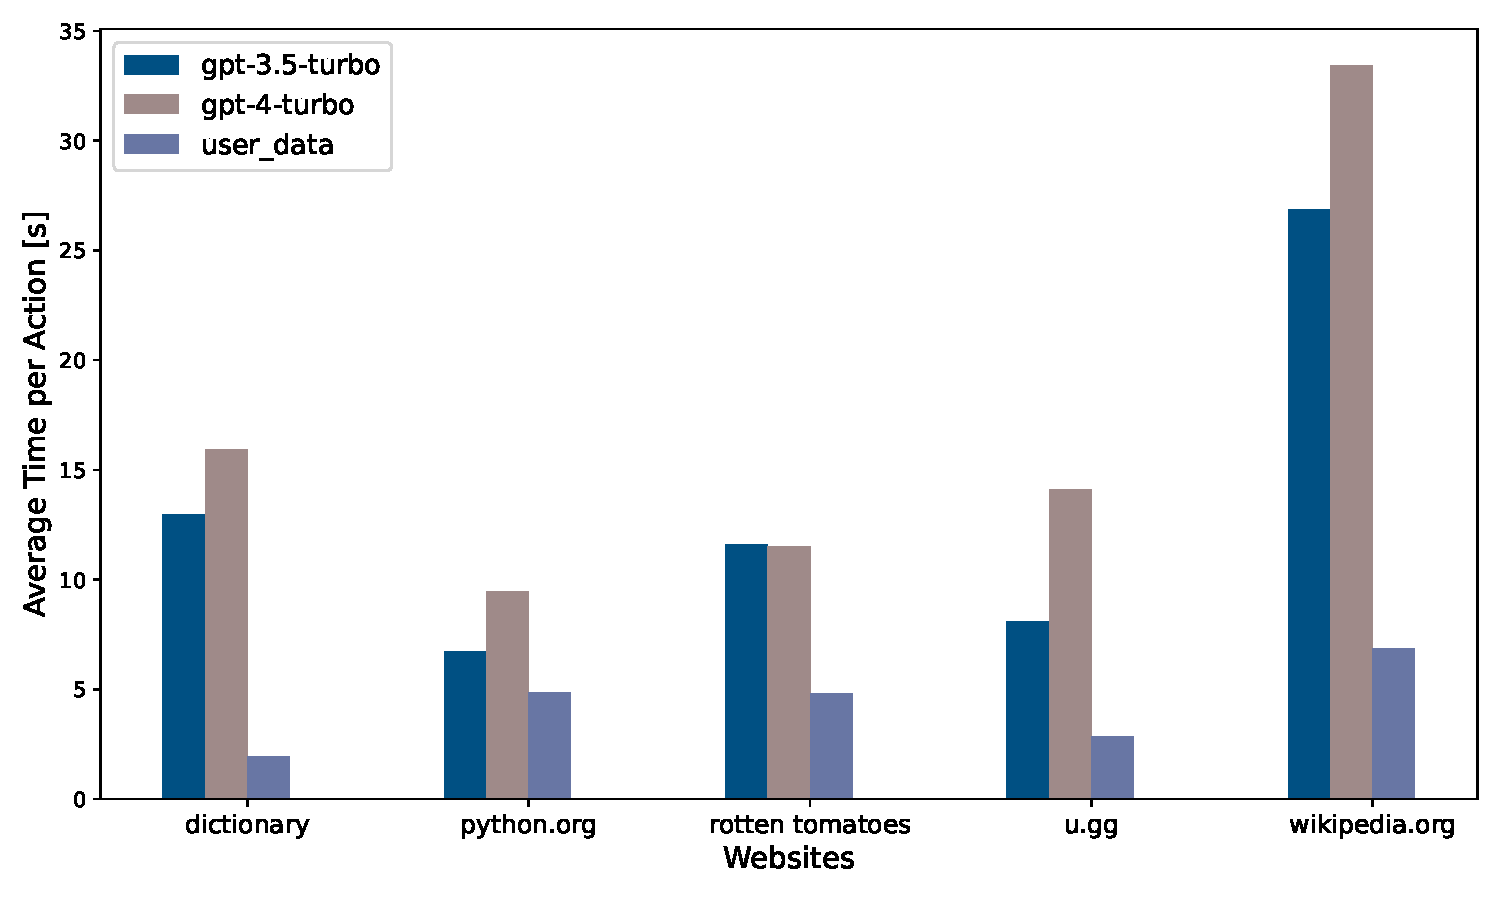
\includegraphics[width=1\textwidth]{obrazky-figures/average_time_per_action_comparison.pdf}
    \caption{average time per action}
    \label{tfa}
\end{figure}

Figure \ref{tfa} shows large differences between the LLM models and human data. Because the simulator is designed not to model a frequency of actions in a human-like sense and the LLM models are slow, the time to do an action is higher.

\subsection{Evaluation of Web navigation}

The last experiment explores the differences and similarities between humans' web navigation and the simulator. The Sankey diagram was created from URLs in a given action using a Jupiter notebook. The Diagram shows transitions between different pages for each of the simulations or human recordings.

\subsubsection{Wikipedia.org}

Figure \ref{sankey_wikipedia_llm} shows the navigation of the simulator throughout the simulation. The results show that the decisions of the LLM tend to be the same, And all of the simulations end on a page containing information about Václav Havel. The diagram shows four different paths towards the final page. 


\begin{figure}[H]
    \centering
    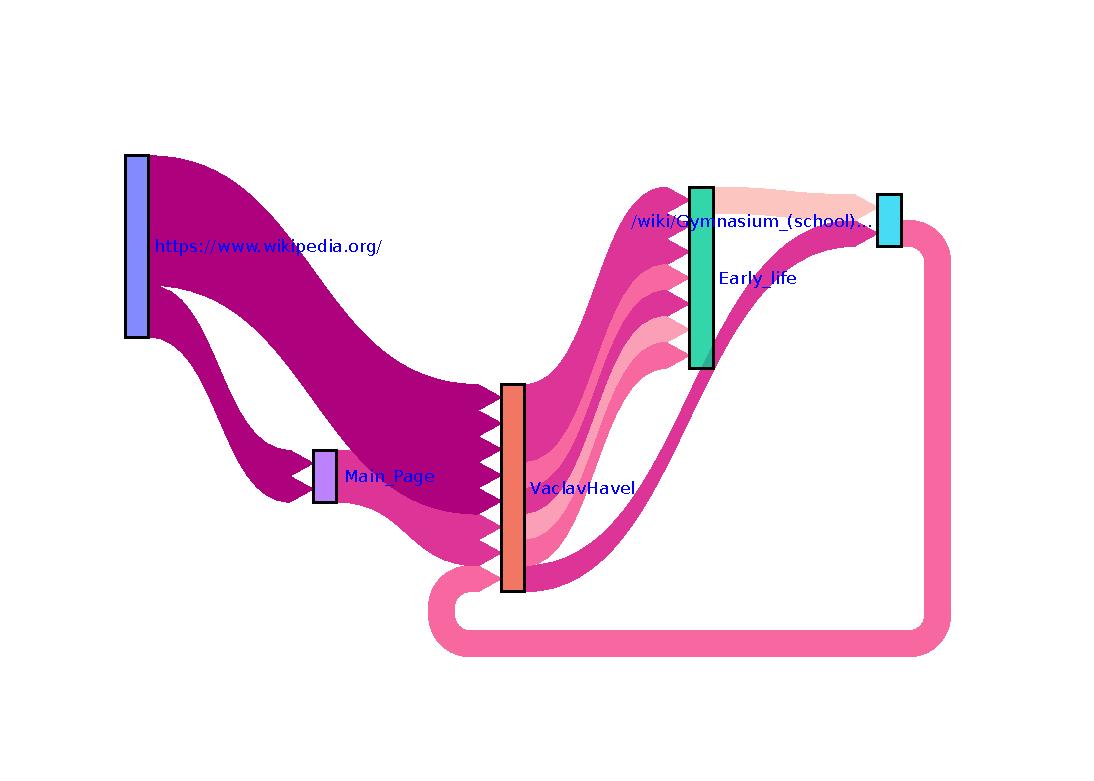
\includegraphics[width=\textwidth]{obrazky-figures/sankey_wikipedia_llm.pdf}
    \caption{Sankey diagram of LLM navigation on Wikipedia.org}
    \label{sankey_wikipedia_llm}
\end{figure}

Figure \ref{sankey_wikipedia_human} displays the path of humans throughout the webpage. Most of the Human respondents followed a similar path. The diagram shows that most of the paths have a direct transition between the main page and the final page containing the information for the goal accomplishment. 

\begin{figure}[H]
    \centering
    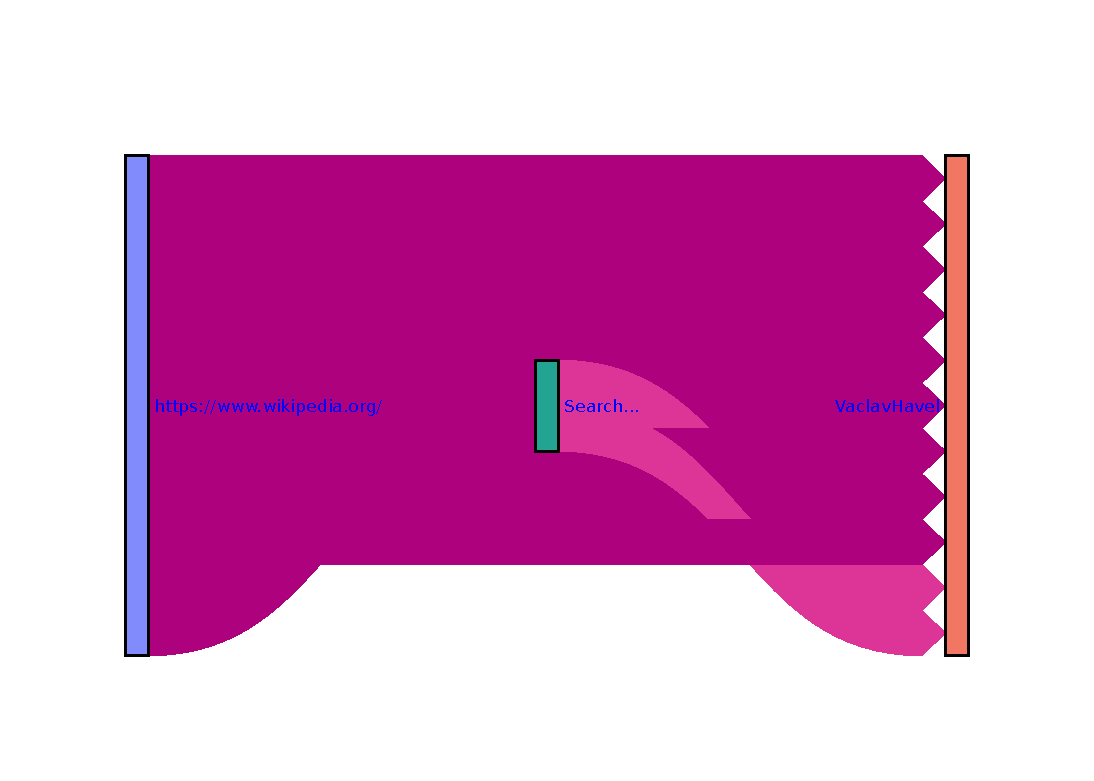
\includegraphics[width=\textwidth]{obrazky-figures/sankey_wikipedia_human.pdf}
    \caption{Sankey diagram of human navigation on Wikipedia.org}
    \label{sankey_wikipedia_human}
\end{figure}

Completing the goal on the Wikipedia page does not provide many different possibilities. Therefore, the graphs do not have that many nodes; however, there are still certain differences. The differences are in the number of unique pages visited before the goal is accomplished. Furthermore, it shows that the human paths are more consistent on the Wikipedia page, whereas the LLM models differ for certain runs.

\subsubsection{U.gg}

Because the u.gg website is made to find information about characters in a video game in a short amount of time, the path to accomplishing the goal is straightforward. Most of the successful paths contain only two or three unique URLs. 

Figure \ref{sankey_ugg_llm} shows the paths of the simulations. As seen in the diagram, the URLs between the simulations are the same. The portion of the simulations only needed to make a transition to one URL to be able to complete the goal. The results show that the LLM chose similar actions for the simulation.

\begin{figure}[H]
    \centering
    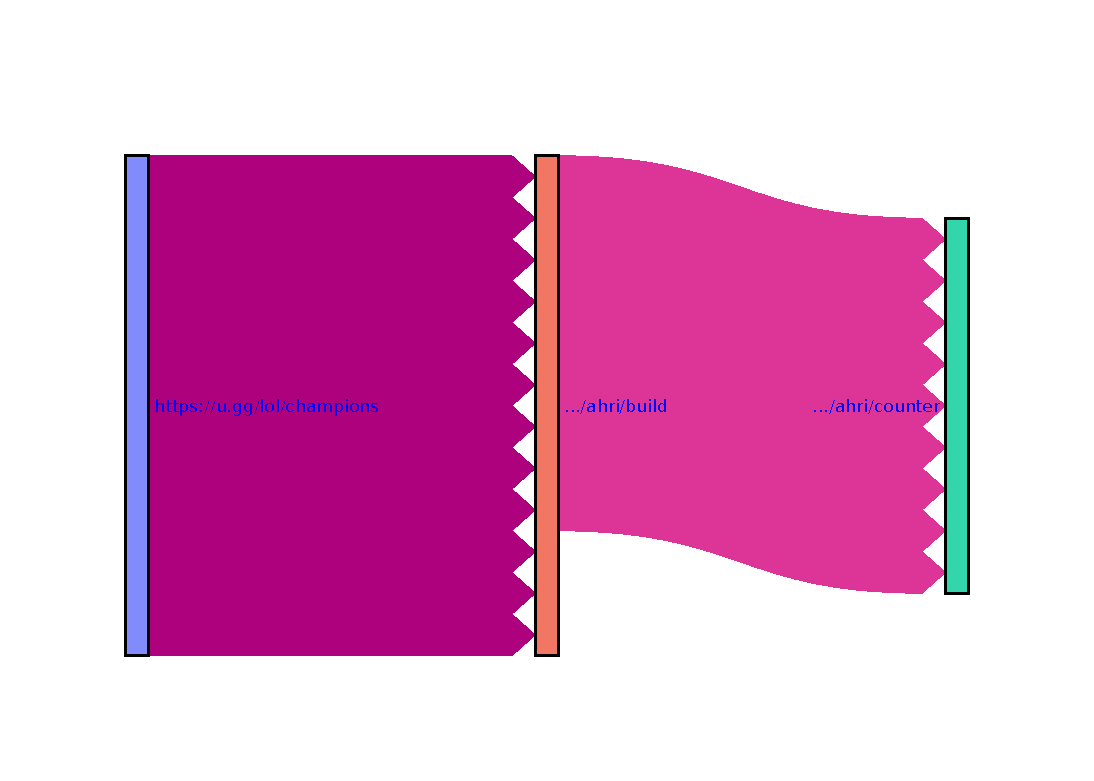
\includegraphics[width=\textwidth]{obrazky-figures/sankey_ugg_llm.pdf}
    \caption{Sankey diagram of LLM navigation on u.gg}
    \label{sankey_ugg_llm}
\end{figure}

Figure \ref{sankey_ugg_human} shows a similar number of different paths with certain cases where the human respondents visited additional websites. Most of the humans chose the same approach as the simulator.  

\begin{figure}[H]
    \centering
    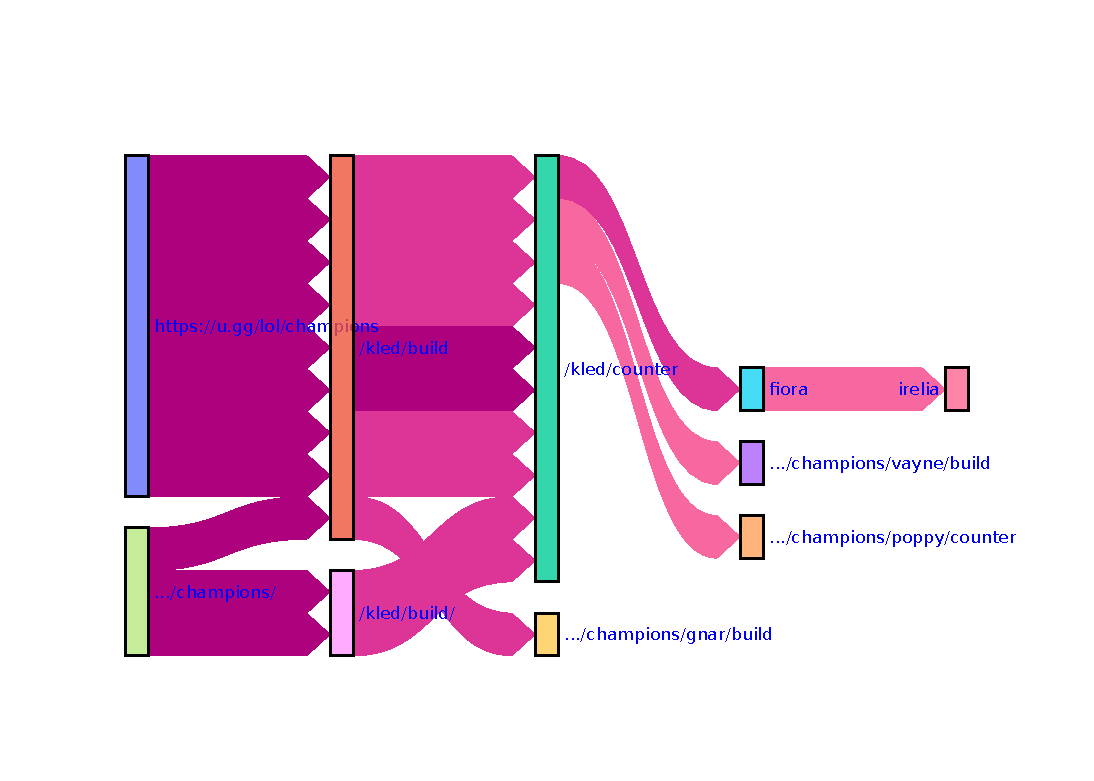
\includegraphics[width=\textwidth]{obrazky-figures/sankey_ugg_human.pdf}
    \caption{Sankey diagram of human navigation on u.gg}
    \label{sankey_ugg_human}
\end{figure}

Both diagrams show similar results for the website u.gg. The human diagram shows four cases where humans visited an additional page with a unique URL that was not necessarily needed to complete the goal.

\subsubsection{Python.org}

Figure \ref{sankey_python_llm} shows small variations in the different simulator runs. The LLMs were able to make accurate decisions in a consistent way. However, the lack of variation shows that the simulator does not simulate all kinds of possible human behaviors. 

\begin{figure}[H]
    \centering
    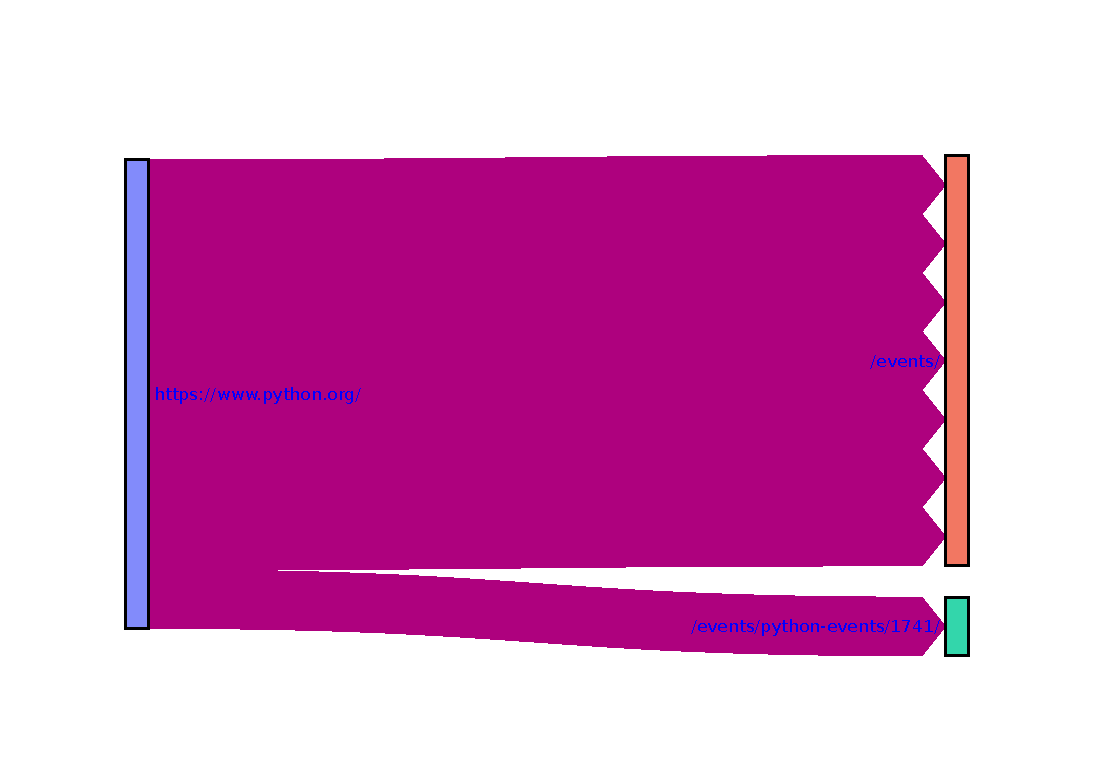
\includegraphics[width=\textwidth]{obrazky-figures/sankey_python_llm.pdf}
    \caption{Sankey diagram of LLM navigation on python.org}
    \label{sankey_python_llm}
\end{figure}

Figure \ref{sankey_python_human} displays human navigation on the website. The Sankey diagram shows very chaotic web navigation. There are a lot of humans who choose different approaches to accomplishing their goals.

\begin{figure}[H]
    \centering
    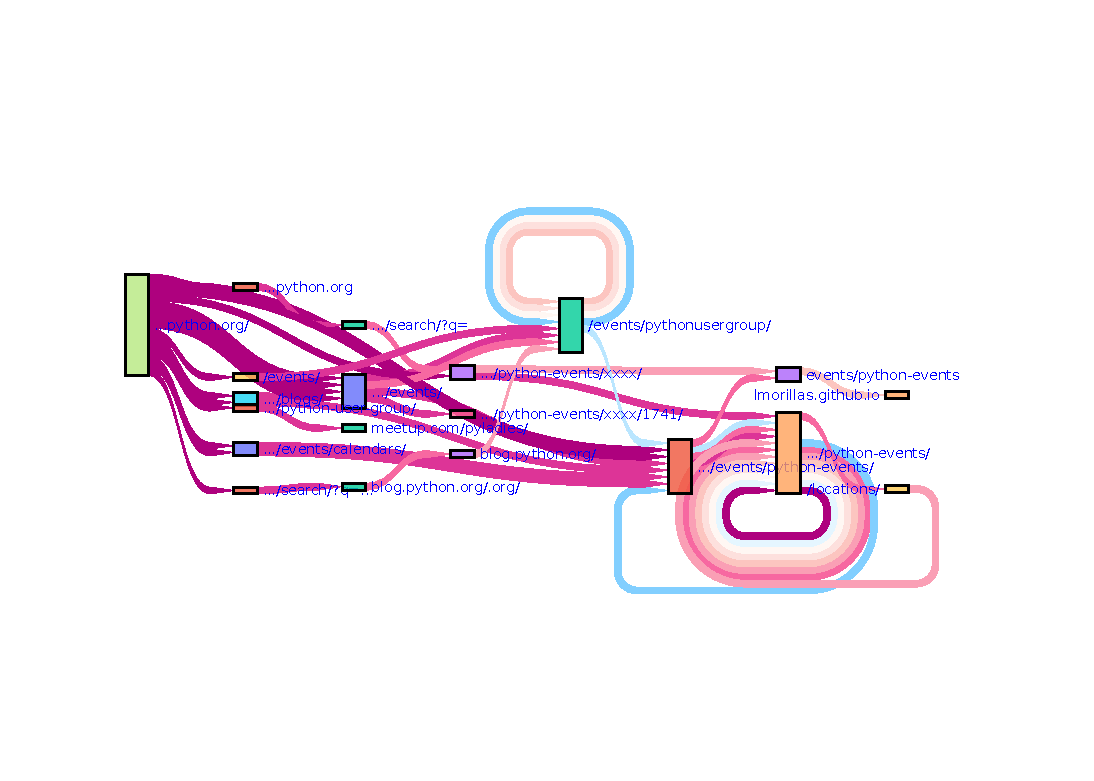
\includegraphics[width=\textwidth]{obrazky-figures/sankey_python_human.pdf}
    \caption{Sankey diagram of human navigation on Python.org}
    \label{sankey_python_human}
\end{figure}

The results on the Python.org website show a large difference between the number of variants of humans and the simulator. This result can be attributed to the fact that the Python.org website allows for multiple of ways how to get to a page that contains information about the upcoming events and has multiple pages with different URLs that contain the information. Furthermore, the example with Python.org shows that the simulator is incapable of automatic variations between the runs. It usually finds the most optimal way how to accomplish the goal.

\subsubsection{Dictionary.cambridge.org}

The dictionary.cambridge.org website uses a search bar to find definitions. Therefore, its navigation is simple. Figure \ref{sankey_dictionary_llm} shows that all simulation runs were the same regarding the transitions between the different URLs. Additionally, Figure \ref{sankey_dictionary_human} shows the same results for the human respondents. The Dictionary site shows its simplicity and no evident differences in the navigation between the LLMs and humans. 

\begin{figure}[H]
    \centering
    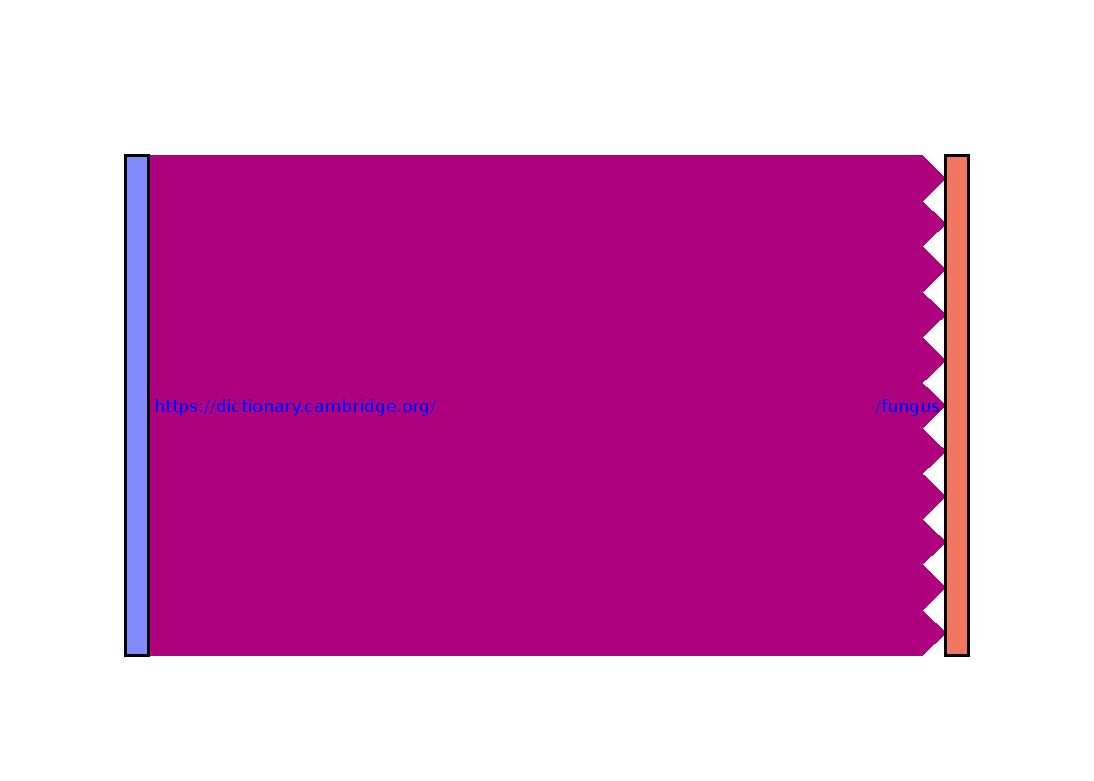
\includegraphics[width=\textwidth]{obrazky-figures/sankey_dictionary_llm.pdf}
    \caption{Sankey diagram of LLM navigation on Cambridge.Dictionary.org}
    \label{sankey_dictionary_llm}
\end{figure}

\begin{figure}[H]
    \centering
    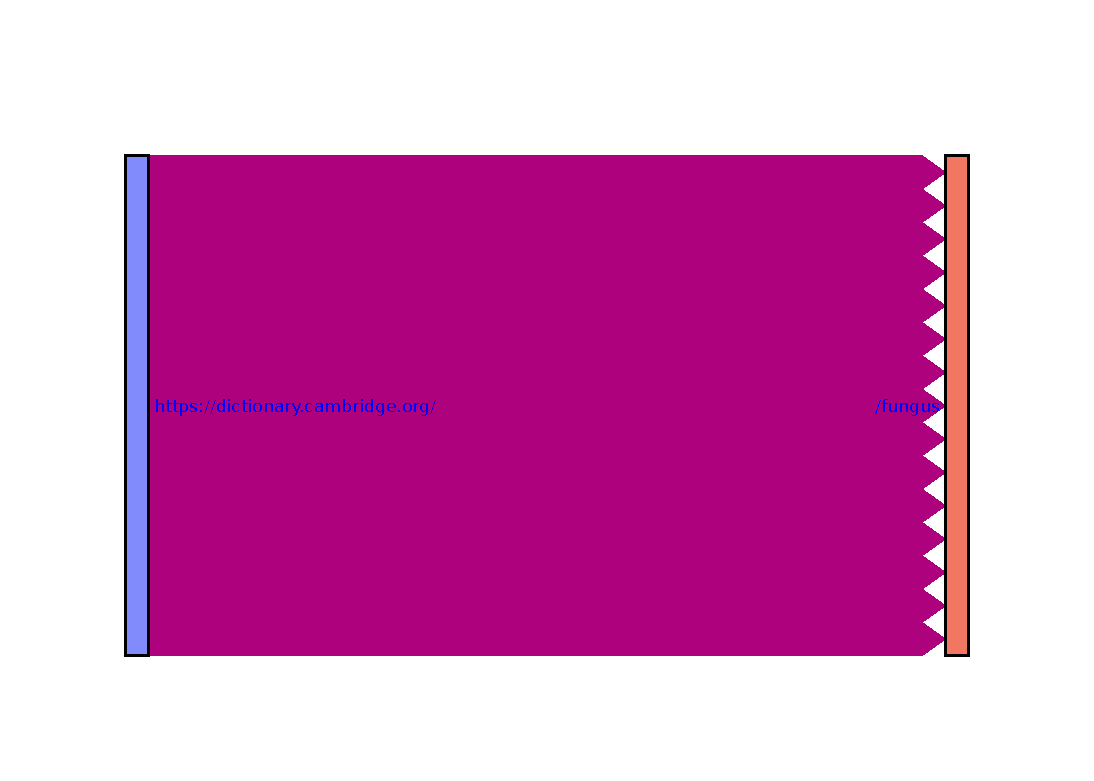
\includegraphics[width=\textwidth]{obrazky-figures/sankey_dictionary_human.pdf}
    \caption{Sankey diagram of Human navigation on Cambridge.Dictionary.org}
    \label{sankey_dictionary_human}
\end{figure}

\subsubsection{Rottentomatoes.com}

Navigation on rottentomatoes.org shows navigation for bot the LLMs and the human respondents. The website has a searchbar that is the only way to retrieve information about a specific film. 

Figure \ref{sankey_tomatoes_llm} displays the navigation of the simulator with a consistent selection of transitions between the URLs. Because of the design of the website, there are not many other ways how to navigate the website to accomplish the goal. 

\begin{figure}[H]
    \centering
    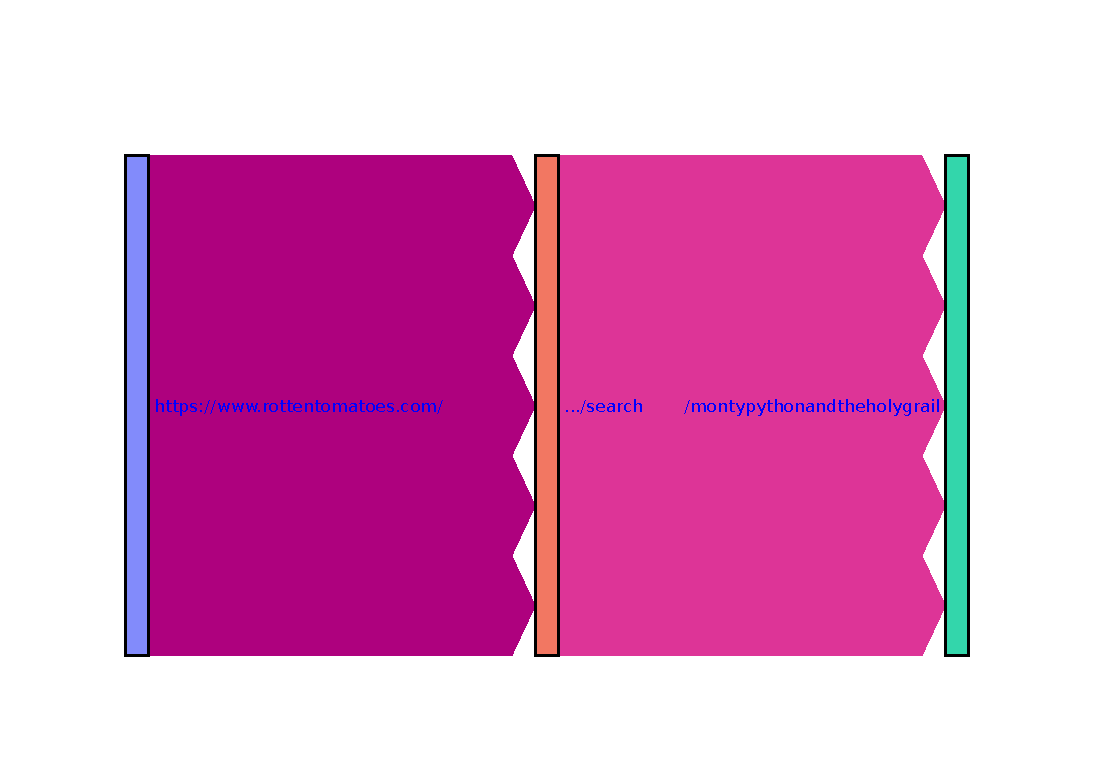
\includegraphics[width=\textwidth]{obrazky-figures/sankey_rotten_tomatoes_llm.pdf}
    \caption{Sankey diagram of LLM navigation on rottentomatoes.org}
    \label{sankey_tomatoes_llm}
\end{figure}

Figure \ref{sankey_tomatoes_human} shows the navigation on the website by humans. The results show that some human respondents were redirected to a website when they misspelled the movie's name. Furthermore, some respondents continued to provide specific details of the director to find their name even though the information could be read from the website. 

\begin{figure}[H]
    \centering
    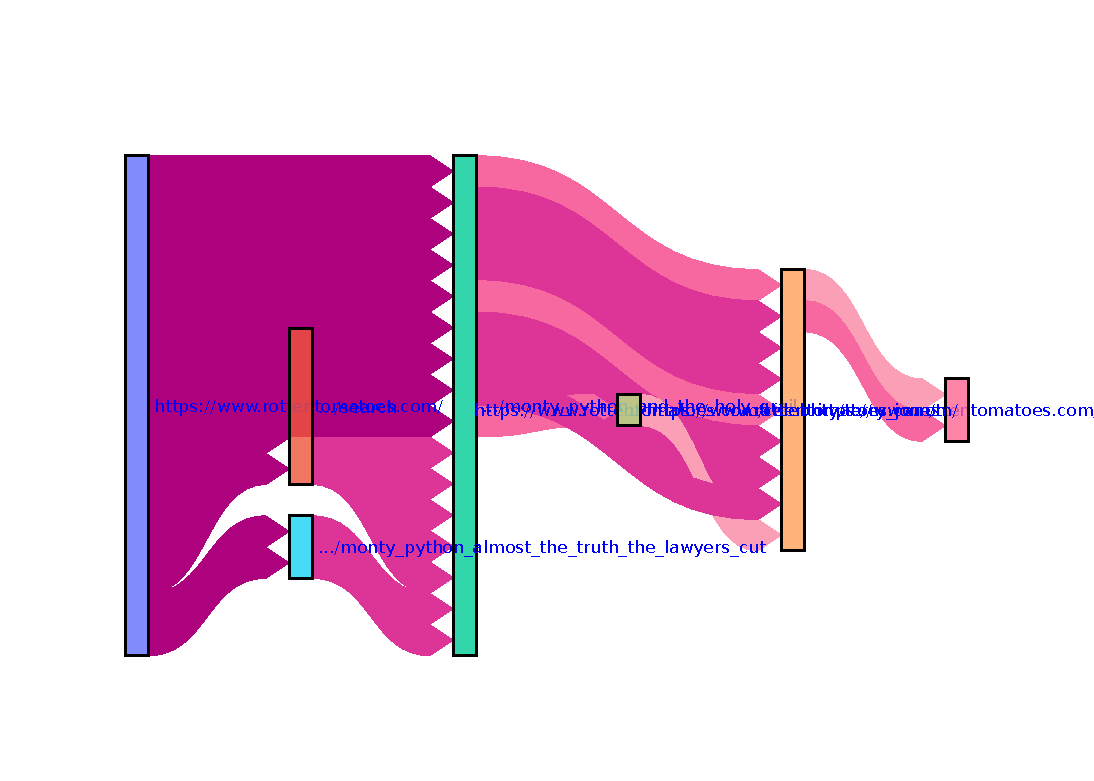
\includegraphics[width=\textwidth]{obrazky-figures/sankey_rotten_tomatoes_human.pdf}
    \caption{Sankey diagram of Human navigation on rottentomatoes.org}
    \label{sankey_tomatoes_human}
\end{figure}

The comparison between LLMs and humans on the website rottentomatoes.com shows that the types of transitions are similar. The difference is mainly caused by some humans misspelling the movie name or by not finishing the goal on the page containing the information needed for the goal completion. 

\chapter{Conclusion}
\label{con}

% co see podarilo
% zajimave poznatky
% vysledky experiment
% future work

To conclude, simulating human web browsing is far from trivial. LLMs represent a~powerful technological advancement capable of solving problems previously thought unsolvable. Utilizing LLMs for the simulation of human behavior presents a~particularly promising avenue.

This work's result is a promising and capable tool for automatic web navigation and goal completion based on the general specification of a goal and website. The proposed architecture and implementation allow for the simulation to work on a~large number of websites. The result shows the usability of LLM models for human simulation and the creation of decision-making applications. The work defines challenges to be tackled when developing LLM-powered tools and shows how to resolve them. 

The results of the experiments show an over 80\% success rate for the GPT 4 Turbo model and a decent success rate for the other model. Together, they show a~high accuracy in comparing Human behavior, showing the proposed tool's capability and similarity to organic traffic. The comparison with human data shows limitations of the proposed tool that can be further improved and mitigated. The results suggest the tool can be helpful in real use cases.

Future research should aim to test the proposed tool on a broader set of websites and compare it to a better dataset of human data. Also, the simulator could be improved to use real-time timeouts between the chosen actions. The tool could be further enhanced to let the LLM model create its own goals and better simulate Human web traffic. With a~dataset of different human personas, the tool could be tested to see if the predefined personas match the actual behavior of a~given persona. Furthermore, the predefined actions can be extended, providing more capabilities. Additionally, the tool can be extended to a different use case that involves automatic web navigation and interaction. 

Ultimately, this path towards creating an advanced web browsing simulator pushes the boundaries of LLM capabilities and opens new pathways for understanding and replicating human-computer interactions that can be used for many use cases. 

% \chapter{Appendix}


%=========================================================================

% For compilation piecewise (see projekt.tex), it is necessary to uncomment it
% \end{document}
  \else
    \input{projekt-01-kapitoly-chapters}
  \fi
  
  % Kompilace po částech (viz výše, nutno odkomentovat a zakomentovat input výše)
  % Compilation piecewise (see above, it is necessary to uncomment it and comment out input above)
  %\subfile{chapters/projekt-01-uvod-introduction}
  % ...
  %\subfile{chapters/projekt-05-zaver-conclusion}

  % Pouzita literatura / Bibliography
  % ----------------------------------------------
\ifslovak
  \makeatletter
  \def\@openbib@code{\addcontentsline{toc}{chapter}{Literatúra}}
  \makeatother
  \bibliographystyle{bib-styles/Pysny/skplain}
\else
  \ifczech
    \makeatletter
    \def\@openbib@code{\addcontentsline{toc}{chapter}{Literatura}}
    \makeatother
    \bibliographystyle{bib-styles/Pysny/czplain}
  \else 
    \makeatletter
    \def\@openbib@code{\addcontentsline{toc}{chapter}{Bibliography}}
    \makeatother
    \bibliographystyle{bib-styles/Pysny/enplain}
  %  \bibliographystyle{alpha}
  \fi
\fi
  \begin{flushleft}
  \bibliography{projekt-20-literatura-bibliography}
  \end{flushleft}

  % vynechani stranky v oboustrannem rezimu
  % Skip the page in the two-sided mode
  \iftwoside
    \cleardoublepage
  \fi

  % Prilohy / Appendices
  % ---------------------------------------------
  \appendix
\ifczech
  \renewcommand{\appendixpagename}{Přílohy}
  \renewcommand{\appendixtocname}{Přílohy}
  \renewcommand{\appendixname}{Příloha}
\fi
\ifslovak
  \renewcommand{\appendixpagename}{Prílohy}
  \renewcommand{\appendixtocname}{Prílohy}
  \renewcommand{\appendixname}{Príloha}
\fi
%  \appendixpage

% vynechani stranky v oboustrannem rezimu
% Skip the page in the two-sided mode
%\iftwoside
%  \cleardoublepage
%\fi

\ifslovak
%  \section*{Zoznam príloh}
%  \addcontentsline{toc}{section}{Zoznam príloh}
\else
  \ifczech
%    \section*{Seznam příloh}
%    \addcontentsline{toc}{section}{Seznam příloh}
  \else
%    \section*{List of Appendices}
%    \addcontentsline{toc}{section}{List of Appendices}
  \fi
\fi
  \startcontents[chapters]
  \setlength{\parskip}{0pt} 
  % seznam příloh / list of appendices
  % \printcontents[chapters]{l}{0}{\setcounter{tocdepth}{2}}
  
  \ifODSAZ
    \setlength{\parskip}{0.5\bigskipamount}
  \else
    \setlength{\parskip}{0pt}
  \fi
  
  % vynechani stranky v oboustrannem rezimu
  \iftwoside
    \cleardoublepage
  \fi
  
  % Přílohy / Appendices
  \ifenglish
    % This file should be replaced with your file with an appendices (headings below are examples only)

% For compilation piecewise (see projekt.tex), it is necessary to uncomment it and change
%\documentclass[../projekt.tex]{subfiles}
%\begin{document}

% Placing of table of contents of the memory media here should be consulted with a supervisor
\chapter{Contents of the included storage media}

\dirtree{%
.1 SD\_card/.
.2 data\_humans/.
.2 experiment\_data/.
.2 experiment\_data\_requests/.
.2 figures/.
.2 src/.
.3 \_\_init\_\_.py.
.3 chains.py.
.3 llm\_provider.py.
.3 logger.py.
.3 simulation.py.
.3 web.py.
.2 \_\_init\_\_.py.
.2 app.py.
.2 benchmark.ipynb.
.2 benchmark.py.
.2 config.json.
.2 RADME.md.
.2 doc.
.3 BP.pdf.
.3 src/.
}

%\chapter{Manual}

%\chapter{Configuration file}

%\chapter{Scheme of RelaxNG configuration file}

%\chapter{Poster}

% \chapter{How to use this template}
% \label{jak}


  \else
    % Tento soubor nahraďte vlastním souborem s přílohami (nadpisy níže jsou pouze pro příklad)

% Pro kompilaci po částech (viz projekt.tex), nutno odkomentovat a upravit
%\documentclass[../projekt.tex]{subfiles}
%\begin{document}

% Umístění obsahu paměťového média do příloh je vhodné konzultovat s vedoucím
%\chapter{Obsah přiloženého paměťového média}

%\chapter{Manuál}

%\chapter{Konfigurační soubor}

%\chapter{RelaxNG Schéma konfiguračního souboru}

%\chapter{Plakát}

\chapter{Jak pracovat s touto šablonou}
\label{jak}

V této příloze je uveden popis jednotlivých částí šablony, po kterém následuje stručný návod, jak s touto šablonou pracovat. Pokud po jejím přečtení k šabloně budete mít nějaké dotazy, připomínky apod., neváhejte a napište na e-mail \texttt{sablona@fit.vutbr.cz}.

\section*{Popis částí šablony}

Po rozbalení šablony naleznete následující soubory a adresáře:
\begin{DESCRIPTION}
  \item [bib-styles] Styly literatury (viz níže). 
  \item [obrazky-figures] Adresář pro Vaše obrázky. Nyní obsahuje \texttt{placeholder.pdf} (tzv. TODO obrázek, který lze použít jako pomůcku při tvorbě technické zprávy), který se s prací neodevzdává. Název adresáře je vhodné zkrátit, aby byl jen ve zvoleném jazyce.
  \item [template-fig] Obrázky šablony (znak VUT).
  \item [fitthesis.cls] Šablona (definice vzhledu).
  \item [Makefile] Makefile pro překlad, počítání normostran, sbalení apod. (viz níže).
  \item [projekt-01-kapitoly-chapters.tex] Soubor pro Váš text (obsah nahraďte).
  \item [projekt-20-literatura-bibliography.bib] Seznam literatury (viz níže).
  \item [projekt-30-prilohy-appendices.tex] Soubor pro přílohy (obsah nahraďte).
  \item [projekt.tex] Hlavní soubor práce -- definice formálních částí.
\end{DESCRIPTION}

Styl literatury v šabloně je od Ing. Radka Pyšného \cite{Pysny}, jehož práce byla vylepšena prof. Adamem Heroutem, dr. Jaroslavem Dytrychem a panem Karlem Hanákem tak, aby odpovídala normě a podporovala všechny často využívané typy citací. Jeho dokumentaci naleznete v příloze \ref{priloha-priklady-citaci}.

\begin{samepage}
Makefile kromě překladu do PDF nabízí i další funkce:
\begin{itemize}
  \item přejmenování souborů (viz níže),
  \item počítání normostran,
  \item spuštění vlny pro doplnění nezlomitelných mezer,
  \item sbalení výsledku pro odeslání vedoucímu ke kontrole (zkontrolujte, zda sbalí všechny Vámi přidané soubory, a případně doplňte).
\end{itemize}
\end{samepage}

Nezapomeňte, že vlna neřeší všechny nezlomitelné mezery. Vždy je třeba manuální kontrola, zda na konci řádku nezůstalo něco nevhodného -- viz Internetová jazyková příručka\footnote{Internetová jazyková příručka \url{http://prirucka.ujc.cas.cz/?id=880}}.

\paragraph {Pozor na číslování stránek!} Pokud má obsah 2 strany a na 2. jsou jen \uv{Přílohy} a~\uv{Seznam příloh} (ale žádná příloha tam není), z nějakého důvodu se posune číslování stránek o 1 (obsah \uv{nesedí}). Stejný efekt má, když je na 2. či 3. stránce obsahu jen \uv{Literatura} a~je možné, že tohoto problému lze dosáhnout i jinak. Řešení je několik (od~úpravy obsahu, přes nastavení počítadla až po sofistikovanější metody). \textbf{Před odevzdáním proto vždy překontrolujte číslování stran!}


\section*{Doporučený postup práce se šablonou}

\begin{enumerate}
  \item \textbf{Zkontrolujte, zda máte aktuální verzi šablony.} Máte-li šablonu z předchozího roku, na stránkách fakulty již může být novější verze šablony s~aktualizovanými informacemi, opravenými chybami apod.
  \item \textbf{Zvolte si jazyk}, ve kterém budete psát svoji technickou zprávu (česky, slovensky nebo anglicky) a svoji volbu konzultujte s vedoucím práce (nebyla-li dohodnuta předem). Pokud Vámi zvoleným jazykem technické zprávy není čeština, nastavte příslušný parametr šablony v souboru projekt.tex (např.: \verb|document|\verb|class[english]{fitthesis}| a přeložte prohlášení a poděkování do~angličtiny či slovenštiny.
  \item \textbf{Přejmenujte soubory.} Po rozbalení je v šabloně soubor \texttt{projekt.tex}. Pokud jej přeložíte, vznikne PDF s technickou zprávou pojmenované \texttt{projekt.pdf}. Když vedoucímu více studentů pošle \texttt{projekt.pdf} ke kontrole, musí je pracně přejmenovávat. Proto je vždy vhodné tento soubor přejmenovat tak, aby obsahoval Váš login a (případně zkrácené) téma práce. Vyhněte se však použití mezer, diakritiky a speciálních znaků. Vhodný název může být např.: \uv{\texttt{xlogin00-Cisteni-a-extrakce-textu.tex}}. K přejmenování můžete využít i přiložený Makefile:
\begin{verbatim}
make rename NAME=xlogin00-Cisteni-a-extrakce-textu
\end{verbatim}
  \item Vyplňte požadované položky v souboru, který byl původně pojmenován \texttt{projekt.tex}, tedy typ, rok (odevzdání), název práce, svoje jméno, ústav (dle zadání), tituly a~jméno vedoucího, abstrakt, klíčová slova a další formální náležitosti.
  \item Nahraďte obsah souborů s kapitolami práce, literaturou a přílohami obsahem svojí technické zprávy. Jednotlivé přílohy či kapitoly práce může být výhodné uložit do~samostatných souborů -- rozhodnete-li se pro toto řešení, je doporučeno zachovat konvenci pro názvy souborů, přičemž za číslem bude následovat název kapitoly. 
  \item Nepotřebujete-li přílohy, zakomentujte příslušnou část v \texttt{projekt.tex} a příslušný soubor vyprázdněte či smažte. Nesnažte se prosím vymyslet nějakou neúčelnou přílohu jen proto, aby daný soubor bylo čím naplnit. Vhodnou přílohou může být obsah přiloženého paměťového média.
  \item Smažte soubory s kapitolami a přílohami pro jazyk, který jste nevyužili (s nebo bez \texttt{-en}).
  \item Zadání, které si stáhnete v PDF z IS VUT (odkaz \uv{Zadání pro vložení do práce} či \uv{Thesis assignment}), uložte do souboru \texttt{zadani.pdf} a povolte jeho vložení do práce parametrem šablony v \texttt{projekt.tex} (\verb|document|\verb|class[zadani]{fitthesis}|).
  \item Nechcete-li odkazy tisknout barevně (bez konzultace s vedoucím příliš nedoporučuji), budete pro tisk vytvářet druhé PDF s tím, že nastavíte parametr šablony pro tisk: (\verb|document|\verb|class[zadani,print]{fitthesis}|). Budete-li tisknout barevně, místo \texttt{print} použijte parametr \texttt{cprint}. Barevné logo se nesmí tisknout černobíle!
  \item Vzor desek, do kterých bude práce vyvázána, si vygenerujte v informačním systému fakulty u zadání. Pro disertační práci lze zapnout parametrem v šabloně \texttt{cover} (více naleznete v souboru \texttt{fitthesis.cls}).
  \item Nezapomeňte, že zdrojové soubory i (obě verze) PDF musíte odevzdat na CD či jiném médiu přiloženém k technické zprávě.
\end{enumerate}

Obsah práce se generuje standardním příkazem \tt \textbackslash tableofcontents \rm (zahrnut v šabloně). Přílohy jsou v něm uvedeny úmyslně.

\subsection*{Pokyny pro oboustranný tisk}
\begin{itemize}
\item \textbf{Oboustranný tisk je doporučeno konzultovat s vedoucím práce.}
\item Je-li práce tištěna oboustranně a její tloušťka je menší než tloušťka desek, nevypadá to dobře.
\item Zapíná se parametrem šablony: \verb|\document|\verb|class[twoside]{fitthesis}|
\item Po vytištění oboustranného listu zkontrolujte, zda je při prosvícení sazební obrazec na obou stranách na stejné pozici. Méně kvalitní tiskárny s duplexní jednotkou mají často posun o 1--3 mm. Toto může být u některých tiskáren řešitelné tak, že vytisknete nejprve liché stránky, pak je dáte do stejného zásobníku a vytisknete sudé.
\item Za titulním listem, obsahem, literaturou, úvodním listem příloh, seznamem příloh a případnými dalšími seznamy je třeba nechat volnou stránku, aby následující část začínala na liché stránce (\texttt{\textbackslash cleardoublepage}).
\item  Konečný výsledek je nutné pečlivě překontrolovat.
\end{itemize}

\subsection*{Styl odstavců}

Odstavce se zarovnávají do bloku a pro jejich formátování existuje více metod. U papírové literatury je častá metoda s~použitím odstavcové zarážky, kdy se u~jednotlivých odstavců textu odsazuje první řádek odstavce asi o~jeden až dva čtverčíky, tedy přibližně o~dvě šířky velkého písmene M základního textu (vždy o~stejnou, předem zvolenou hodnotu). Poslední řádek předchozího odstavce a~první řádek následujícího odstavce se v~takovém případě neoddělují svislou mezerou. Proklad mezi těmito řádky je stejný jako proklad mezi řádky uvnitř odstavce \cite{fitWeb}.

Další metodou je odsazení odstavců, které je časté u elektronické sazby textů. První řádek odstavce se při této metodě neodsazuje a mezi odstavce se vkládá vertikální mezera o~velikosti 1/2 řádku. Obě metody lze v kvalifikační práci použít, nicméně často je vhodnější druhá z uvedených metod. Metody není vhodné kombinovat.

Jeden z výše uvedených způsobů je v šabloně nastaven jako výchozí, druhý můžete zvolit parametrem šablony \uv{\tt odsaz\rm }.

\subsection*{Užitečné nástroje}
\label{nastroje}

Následující seznam není výčtem všech využitelných nástrojů. Máte-li vyzkoušený osvědčený nástroj, neváhejte jej využít. Pokud však nevíte, který nástroj si zvolit, můžete zvážit některý z následujících:

\begin{description}
	\item[\href{http://miktex.org/download}{MikTeX}] \LaTeX{} pro Windows -- distribuce s jednoduchou instalací a vynikající automatizací stahování balíčků. MikTex obsahuje i vlastní editor, ale spíše doporučuji TeXstudio.
	\item[\href{http://texstudio.sourceforge.net/}{TeXstudio}] Přenositelné GUI pro \LaTeX{} s otevřeným zdrojovým kódem (opensource).  Ctrl+klik umožňuje přepínat mezi zdrojovým textem a PDF. Má integrovanou kontrolu pravopisu\footnote{Českou kontrolu pravopisu lze doinstalovat z \url{https://extensions.openoffice.org/de/project/czech-dictionary-pack-ceske-slovniky-cs-cz}}, zvýraznění syntaxe apod. Pro jeho využití je nejprve potřeba nainstalovat MikTeX, případně jinou \LaTeX ovou distribuci.
	\item[\href{http://www.winedt.com/}{WinEdt}] Ve Windows je dobrá kombinace WinEdt + MiKTeX. WinEdt je GUI pro Windows, pro jehož využití je nejprve potřeba nainstalovat \href{http://miktex.org/download}{MikTeX} či \href{http://www.tug.org/texlive/}{TeX Live}. 
	\item[\href{http://kile.sourceforge.net/}{Kile}] Editor pro desktopové prostředí KDE (Linux). Umožňuje živé zobrazení náhledu. Pro jeho využití je potřeba mít nainstalovaný \href{http://www.tug.org/texlive/}{TeX Live} a Okular. 
	\item[\href{http://jabref.sourceforge.net/download.php}{JabRef}] Pěkný a jednoduchý program v Javě pro správu souborů s bibliografií (literaturou). Není potřeba se nic učit -- poskytuje jednoduché okno a formulář pro editaci položek.
	\item[\href{https://inkscape.org/en/download/}{InkScape}] Přenositelný opensource editor vektorové grafiky (SVG i PDF). Vynikající nástroj pro tvorbu obrázků do odborného textu. Jeho ovládnutí je obtížnější, ale výsledky stojí za to.
	\item[\href{https://git-scm.com/}{GIT}] Vynikající pro týmovou spolupráci na projektech, ale může výrazně pomoci i jednomu autorovi. Umožňuje jednoduché verzování, zálohování a přenášení mezi více počítači.
	\item[\href{http://www.overleaf.com/}{Overleaf}] Online nástroj pro \LaTeX{}. Přímo zobrazuje náhled a umožňuje jednoduchou spolupráci (vedoucí může průběžně sledovat psaní práce), vyhledávání ve zdrojovém textu či ve vygenerovaném PDF, kontrolu pravopisu apod. Zdarma jej však lze využít pouze s určitými omezeními (někomu stačí na disertaci, jiný na ně může narazit i při psaní bakalářské práce) a pro dlouhé texty je pomalejší. FIT VUT v Brně má pro studenty i~zaměstnance licenci, kterou si lze aktivovat na \url{https://www.overleaf.com/edu/but}.
\end{description}

Pozn.: Overleaf nepoužívá Makefile v šabloně -- aby překlad fungoval, je v menu nutné zvolit \tt projekt.tex \rm jako hlavní dokument.

\chapter{Psaní anglického textu}
\label{anglicky}
Tato příloha je převzata ze stránek doc. Černockého \cite{CernockyEnglish}.

Spousta lidí píše zprávy k projektům anglicky (a to je dobře!), ale dělá v nich spoustu zbytečných chyb (a to je špatně). Nejsem angličtinář, ale tento jazyk už nějakých pár let používám k psaní, čtení i komunikaci -- tato příloha obsahuje pár důležitých věcí. Pokud chcete napsat práci nebo článek opravdu 100\,\% dobře, nezbude Vám než si najmout rodilého mluvčího (a to by měl by být trochu technicky zdatný a aspoň trochu rozumět tomu, co píšete, ať to neskončí ještě hůř \ldots).

\section*{Obecně}

\begin{itemize}
  \item{Předtím, než budete sami něco psát, si přečtěte pár anglických technických článků a~zkuste si zapamatovat a získat \uv{obecný pocit}, jak se to píše.}
  \item{Používejte vždy korektor pravopisu -- zabudovaný ve Wordu, nebo v OpenOffice, pokud děláte na Linuxu, tak ISPELL a další (většina editorů pro \LaTeX{} má již kontrolu pravopisu integrovanou).}
  \item{Používejte korektor gramatiky. Nevím, jestli je nějaký dostupný na Linuxu, ale ten ve Wordu celkem slušně funguje a pokud Vám něco zelené podtrhne, je tam většinou opravdu chyba. Můžete do něj nakopírovat i zdrojový text pro \LaTeX{}, opravit, a pak uložit opět jako čistý text. Pokud používáte vim, je tam zabudovaný také a zvládne jak překlepy, tak základní gramatiku. V dokumentu \texttt{diplomka.tex} na první řádek napište: 
  \begin{verbatim}
    % vim:spelllang=en_us:spell
  \end{verbatim}
  (případně \texttt{en\_gb} pro OED angličtinu)
  \textit{Poznámka editora:} Existuje i velmi dobrý online nástroj Grammarly\footnote{\url{https://www.grammarly.com/}}, který je v základní verzi zdarma. 
  }
  \item{Online slovníky jsou dobré, ale nepoužívejte je slepě. Většinou dají více variant a ne každá je správně.}
  \item{\begin{samepage}Na vyhledávání a zjištění, co bude asi správné, můžete použít Google. Např.: nevíte, jak se řekne \uv{výhoda tohoto přístupu}. Slovník na seznam.cz dá asi 10 variant. Napište je postupně do vyhledávání na googlu:
  \begin{verbatim}
    "advantage of this approach" 1100000 hits
    "privilege of this approach" 6 hits
    "facility of this approach"  16 hits
  \end{verbatim}
  Neříkám, že je to 100\,\% správně, ale je to určité vodítko. Toto se dá použít i~na~dohledání správných spojek (třeba \uv{among two cases} nebo \uv{between two cases}?)\end{samepage}}
\end{itemize}
       
\section*{SVOMPT a shoda}

Struktura anglické věty je SVOPMT: SUBJECT VERB OBJECT MANNER PLACE TIME a přes to nejede vlak! Není volná jako v češtině. Jinak to je maximálně v nějaké divadelní hře, kde je potřeba něco zdůraznit. Hlavně podmět tam musí vždy být, na to se často zapomíná, protože v CZ/SK může být zamlčený nebo nevyjádřený. SVOMPT platí i~ve vedlejších větách!
\begin{verbatim}
  BAD: We have shown that is faster than the other function. 
  GOOD: We have shown that it is faster than the other function. 
\end{verbatim}

\noindent Shoda podmětu s přísudkem -- zní to šíleně, ale dělá se v tom spousta chyb. 

\begin{verbatim}
  he has 
  the users have 
  people were 
\end{verbatim}

\section*{Členy}

Členy v angličtině jsou noční můra a téměř nikdo z nás je nedává dobře. Základní pravidlo je, že když je něco určitého, musí předtím být \uv{the}. Členy musí být určitě u těchto spojení:
\begin{verbatim}
  the first, the second, ...
  the last
  the most (třetí stupeň přídavných jmen a príslovcí) ...
  the whole 
  the following 
  the figure, the table. 
  the left, the right - on the left pannel, from the left to the right ... 
\end{verbatim}

\noindent Naopak člen NESMÍ být, pokud používáte přesné označení obrázku, kapitoly atd.
\begin{verbatim}
  in Figure 3.2
  in Chapter 7
  in Table 6.4
\end{verbatim}

\begin{samepage}
\noindent Pozor na \uv{a} vs. \uv{an}, řídí se to podle výslovnosti a ne podle toho, jak je slovo napsané, takže:
\begin{verbatim}
  an HMM
  an XML
  a universal model
  a user
\end{verbatim}
\end{samepage}

\section*{Slovesa}

Pozor na trpné tvary sloves -- u pravidelných je to většinou bez problémů, u nepravidelných často špatně, typicky
\begin{verbatim}
  packet was sent (ne send)
  approach was chosen (ne choosed)
\end{verbatim}
\noindent \ldots vetšinou to opraví korektor pravopisu, ale někdy ne. 

Pozor na časy, občas je v nich pěkný nepořádek. Pokud něco nějak obecně je, přítomný čas. Pokud jste něco udělali, minulý. Pokud to dalo nějaký výsledek a ten výsledek teď existuje a třeba ho nějak diskutujete, přítomný. Nepoužívejte příliš složité časy jako je předpřítomný a vůbec ne předminulý pokud nevíte přesně, co děláte.
\begin{verbatim}
  JFA is a technique that works for everyone in speaker recognition. 
  We implemented it according to Kenny's recipe in \cite{Kenny}. 
  12000 segments from NIST SRE 2006 were processed. When compared 
  with a GMM baseline, the results are completely bad. 
\end{verbatim}

\section*{Délka vět a struktura}

\begin{itemize}
  \item{Pište kratší věty a souvětí, pokud máte něco na 5 řádků, většinou se to nedá číst.}
  \item{Strukturujte věty pomocí čárek (více než v češtině!), hlavně po úvodu věty, po kterém začíná vlastní věta. Někdy se dává čárka i před \uv{and} (na rozdíl od češtiny).}
\end{itemize}
\begin{verbatim}
  In this chapter, we will investigate ... 
  The first technique did not work, the second did not work as well, 
  and the third one also did not work. 
\end{verbatim}

\section*{Specifika technického textu}

Píšete technický text, proto nepoužívejte zkratky
\begin{verbatim}
  he's
  gonna
  Petr's working on ...
\end{verbatim}
\noindent a podobně. Jediné, které je tolerované, je \uv{doesn't}, ale neuděláte chybu, když napíšete \uv{does not}. 

\begin{samepage}
\noindent V technických textech se spíš používá trpný rod než činný: 
\begin{verbatim}
  BAD: In this chapter, I describe used programming languages. 
  GOOD: In this chapter, used programming languages are described.
\end{verbatim}
\end{samepage}

Pokud už činný použijete, dává se v technických textech spíše \uv{we}, i když na práci děláte sami. \uv{I}, \uv{my} atd. se používají pouze tam, kde jde o to zdůraznit, že jde o Vaši osobu, tedy třeba v závěru nebo v popisu \uv{original claims} v disertaci.

\paragraph{Časté chyby ve slovech}

\begin{itemize}
  \item{Pozor na jeho/její, není to it's, ale its.}
  \item{Obrázek není picture, ale figure. }
  \item{Spojka \uv{než} je \uv{than}, ne \uv{then} -- bigger than this, smaller than this \ldots hrozně častá chyba! \uv{Then} je pak, potom.}
\end{itemize}


\chapter{Checklist} 
\label{checklist}
Tento checklist byl převzat ze šablony pro kvalifikační práce, která je k dispozici na blogu prof. Herouta \cite{Herout}, který s laskavým dovolením využil nápadu dr. Szökeho%
\footnote{\url{http://blog.igor.szoke.cz/2017/04/predstartovni-priprava-letu-neni.html}}. 

Velká bezpečnost letecké dopravy stojí z části na tom, že lidé kolem letadel mají \textbf{checklisty} na úplně každý, třeba rutinní a dobře zažitý, postup. Jako pilot strpí to, že bude trochu za blbce a opravdu tužtičkou do seznamu úkonů odškrtá dokonale zvládnuté akce, vytiskněte si a odškrtejte před odevzdáním diplomky i vy tento checklist a vyhněte se tak častým chybám, které by mohly mít až fatální následky na výsledné hodnocení Vaší práce.

\subsubsection*{Struktura}
\begin{checklist}
	\item Už ze samotných názvů a struktury kapitol je patrné, že bylo splněno zadání.
	\item V textu se nevyskytuje kapitola, která by měla méně než čtyři strany (kromě úvodu a závěru). Pokud ano, radil(a) jsem se o tom s vedoucím a ten to schválil.
\end{checklist}

\subsubsection*{Obrázky a grafy}
\begin{checklist}
	\item Všechny obrázky a tabulky byly zkontrolovány a jsou poblíž místa, odkud jsou z textu odkazovány, takže nebude problém je najít.
	\item Všechny obrázky a tabulky mají takový popisek, že celý obrázek dává smysl sám o~sobě, bez čtení dalšího textu. Vůbec nevadí, když má popisek několik řádků.
	\item Pokud je obrázek převzatý, tak je to v popisku zmíněno: \uv{Převzato z [X].}
	\item Písmenka ve všech obrázcích používají font podobné velikosti, jako je okolní text (ani výrazně větší, ani výrazně menší).
	\item Grafy a schémata jsou vektorově (tj. v PDF).
	\item Snímky obrazovky nepoužívají ztrátovou kompresi (jsou v PNG).
	\item Všechny obrázky jsou odkázány z textu.
	\item Grafy mají popsané osy (název osy, jednotky, hodnoty) a podle potřeby mřížku.
\end{checklist}

\subsubsection*{Rovnice}
\begin{checklist}
	\item Identifikátory a jejich indexy v rovnicích jsou jednopísmenné (kromě nečastých zvláštních případů jako $t_\mathrm{max}$).
	\item Rovnice jsou číslovány.
	\item Za (nebo vzácně před) rovnicí jsou vysvětleny všechny proměnné a funkce, které zatím vysvětleny nebyly.
\end{checklist}

\subsubsection*{Citace}
\begin{checklist}
    \item \textbf{Všechny použité zdroje jsou citovány.}
	\item Adresy URL odkazující na služby, projekty, zdroje, github apod. jsou odkazovány pomocí \verb|\footnote{\url{...}}|.
    \item Všechny citace používají správné typy.
	\item Citace mají autora, název, vydavatele (název konference), rok vydání.  Když některá nemá, je to dobře zdůvodněný zvláštní případ a vedoucí to odsouhlasil.
	\item Je-li ve zdrojových textech programu něco převzaté, je to tam řádně citováno v souladu s licencí.
	\item Je-li podstatná část zdrojových textů programu převzatá, je toto zmíněno v textu práce a je citován zdroj.
\end{checklist}

\subsubsection*{Typografie}
\begin{checklist}
	\item Žádný řádek nepřetéká přes pravý okraj.
	\item Na konci řádku nikde není jednopísmenná předložka (spraví to nedělitelná mezera $\sim$).
	\item Číslo obrázku, tabulky, rovnice, citace není nikde první na novém řádku (spraví to nedělitelná mezera $\sim$).
	\item Před číselným odkazem na poznámku pod čarou nikde není mezera (to jest vždy takto\footnote{příklad poznámky pod čarou}, nikoliv takto \footnote{jiný příklad poznámky pod čarou}).
\end{checklist}

\subsubsection*{Jazyk}
\begin{checklist}
    \item Použil jsem kontrolu pravopisu a v textu nikde nejsou překlepy.
	\item Nechal jsem si text přečíst od (alespoň) jednoho dalšího člověka, který umí dobře česky / anglicky / slovensky.
	\item V práci psané česky nebo slovensky abstrakt zkontroloval někdo, kdo umí opravdu dobře anglicky.
	\item V textu se nikde nepoužívá druhá mluvnická osoba (vy/ty).
	\item Když se v textu vyskytuje první mluvnická osoba (já, my), vždy se popisuje subjektivní záležitost (\textit{rozhodl jsem se}, \textit{navrhl jsem}, \textit{zaměřil jsem se na}, \textit{zjistil jsem} apod.).
	\item V textu se nikde nepoužívají hovorové výrazy.
	\item V českém či slovenském textu se zbytečně nepoužívají anglické výrazy, které mají ustálené české překlady. Např. slovo \textit{defaultní} se nahradí např. slovem \textit{implicitní} nebo \textit{výchozí}.
\end{checklist}

\subsubsection*{Výsledek na datovém médiu, tj. software}
\begin{checklist}
	\item Mám připravené nepřepisovatelné datové médium 
      \begin{itemize}
	  		\item CD-R,
            \item DVD-R,
            \item DVD+R ve formátu ISO9660 (s rozšířením RockRidge a/nebo Jolliet) nebo UDF,
            \item paměťová karta SD (Secure Digital) ve formátu FAT32 nebo exFAT s nastavenou ochranou proti přepisu.
      \end{itemize}
	\item Pokud je výsledek online (služba, aplikace, \dots), URL je viditelně v úvodu a závěru, aby bylo jasné, kde výsledek hledat.
	\item Na médiu nechybí povinné: 
    	\begin{itemize}
    		\item zdrojové kódy (např. Matlab, C/C++, Python, \dots)
            \item knihovny potřebné pro překlad,
            \item přeložené řešení,
            \item PDF s technickou zprávou (je-li pro tisk 2. verze, tak obě),
            \item zdrojový kód zprávy (\LaTeX), 
    	\end{itemize}
        a případně volitelně po dohodě s vedoucím práce
		\begin{itemize}
			\item relevantní (např. testovací) data, 
            \item demonstrační video,
            \item PDF plakátku,
            \item \dots
		\end{itemize}        
	\item Zdrojové kódy jsou refaktorovány, komentovány a označeny hlavičkou s autorstvím, takže se v nich snadno vyzná i někdo další, než sám autor.
    \item Jakákoliv převzatá část zdrojového kódu je řádně citována -- tedy označena úvodním a v případě převzetí více řádků i ukončovacím komentářem. Komentář obsahuje vše, co vyžaduje licence uvedená na webu (vždy je nutné se ji pokusit najít -- např. Stack Overflow\footnote{\url{https://stackoverflow.blog/2009/06/25/attribution-required/}} má striktní pravidla pro citace).
\end{checklist}

\subsubsection*{Odevzdání}

\begin{checklist}
\item Chci práci (na max. 3 roky) utajit? Pokud ano, nejpozději měsíc před termínem odevzdání práce si podám žádost (v IS), ke které přiložím případné stanovisko firmy, jejíž duševní vlastnictví je třeba chránit.
\item Mám splněný minimální počet normostran textu (lze spočítat pomocí Makefile a~odhadem přičíst obrázky). Pokud jsem těsně pod minimem, konzultoval(a) jsem to s~vedoucím.
\item Pokud chci tisknout oboustranně, konzultoval(a) jsem to s~vedoucím a mám správně nastavenou šablonu. Kapitoly začínají na liché stránce.
\item Technickou zprávu mám v deskách z knihařství (min. 1 výtisk, při utajení oba).
\item Za titulním listem práce je zadání (tzn. mám jej stažené z IS a vložené do šablony).
\item V IS jsou abstrakty a klíčová slova.
  \begin{itemize}
    \item V abstraktu a klíčových slovech v IS nejsou zkopírované vlnky pro nezlomitelné mezery.
  \end{itemize}      
\item V IS je PDF práce (s klikatelnými odkazy).
\item Oba výtisky práce jsou podepsané.
\item V jednom (při utajení obou) výtisku práce je paměťové médium, na kterém je fixkou napsaný login (fixku na CD lze zapůjčit v knihovně, na Studijním oddělení nebo až při odevzdání).
\end{checklist}


\chapter{\LaTeX pro začátečníky}
\label{latex}

V této kapitole jsou uvedeny některé často využívané balíčky a příkazy pro \LaTeX{}, které mohou být při tvorbě práce potřeba.

\subsection*{Užitečné balíčky}

Studenti při sazbě textu často řeší stejné problémy. Některé z nich lze vyřešit následujícími balíčky pro \LaTeX:

\begin{itemize}
  \item \verb|amsmath| -- rozšířené možnosti sazby rovnic,
  \item \verb|float, afterpage, placeins| -- úprava umístění obrázků/tabulek (specifikátor \texttt{H}),
  \item \verb|fancyvrb, alltt| -- úpravy vlastností prostředí Verbatim, 
  \item \verb|makecell| -- rozšíření možností tabulek,
  \item \verb|pdflscape, rotating| -- natočení stránky o 90 stupňů (pro obrázek či tabulku),
  \item \verb|hyphenat| -- úpravy dělení slov,
  \item \verb|picture, epic, eepic| -- přímé kreslení obrázků.
\end{itemize}

Některé balíčky jsou využity přímo v šabloně (v dolní části souboru \texttt{fitthesis.cls}). Nahlédnutí do jejich dokumentace může být rovněž velmi užitečné.

Sloupec tabulky zarovnaný vlevo s pevnou šířkou je v šabloně definovaný \uv{L} (používá se jako \uv{p}).

Pro odkazování v rámci textu použijte příkaz \verb|\ref{navesti}|. Podle umístění návěští se bude jednat o~číslo kapitoly, podkapitoly, obrázku, tabulky nebo podobného číslovaného prvku). Pokud chcete odkázat stránku práce, použijte příkaz \verb|pageref{navesti}|. Pro citaci literárního odkazu \verb|\cite{identifikator}|. Pro odkazy na rovnice lze použít příkaz \verb|\eqref{navesti}|.

Znak \,--\, (pomlčka) se V \LaTeX u vkládá jako dvě mínus za sebou: -{}-.

\subsection*{Často využívané příkazy pro \LaTeX{}}
\label{sec:Fragments}

Doporučuji nahlédnout do zdrojového textu této podkapitoly a podívat se, jak jsou následující ukázky vysázeny. Ve zdrojovém textu jsou i pomocné komentáře.

% Sloupec zarovnaný vlevo s pevnou šířkou je v šabloně definovaný "L" (používá se jako p)

Příklad tabulky:
\begin{table}[H]
	\vskip6pt
	\caption{Tabulka hodnocení} 
    \vskip6pt
	\centering
	\begin{tabular}{llr}
		\toprule
		\multicolumn{2}{c}{Jméno} \\
		\cmidrule(r){1-2}
		Jméno & Příjmení & Hodnocení \\
		\midrule
		Jan & Novák & $7.5$ \\
		Petr & Novák & $2$ \\
		\bottomrule
	\end{tabular}
	\label{tab:ExampleTable}
\end{table}

% Ohraničení lze upravit dle potřeby:
% http://latex-community.org/forum/viewtopic.php?f=45&t=24323
% http://tex.stackexchange.com/questions/58163/problem-with-multirow-and-table-cell-borders
% http://tex.stackexchange.com/questions/79369/formatting-table-border-and-text-alignment-in-latex-table

\noindent Příklad rovnice:
\begin{equation}
	\cos^3 \theta =\frac{1}{4}\cos\theta+\frac{3}{4}\cos 3\theta
	\label{eq:rovnice2}
\end{equation}
a dvou horizontálně zarovnaných rovnic: % znak & řídí zarovnání
\begin{align} 
    \label{eq:soustava}
	3x &= 6y + 12 \\
	x &= 2y + 4 
\end{align}

Pokud je třeba rovnici citovat v textu, lze použít příkaz \verb|\eqref|. Například na rovnici výše lze odkázat~\eqref{eq:rovnice2}. Pokud chcete srovnat číslo rovnic u soustavy, lze použít prostředí \texttt{split}:
\begin{equation} \label{eq:soustavaSrovnana}
\begin{split}
	3x &= 6y + 12 \\
	x &= 2y + 4
\end{split}
\end{equation}

Matematické symboly ($\alpha$) a výrazy lze umístit i do textu $\cos\pi=-1$ a mohou být i~v~poznámce pod čarou%
\footnote{Vzorec v poznámce pod čarou: $\cos\pi=-1$}.

Obrázek~\ref{sirokyObrazek} ukazuje široký obrázek složený z více menších obrázků. Klasický rastrový obrázek se vkládá tak, jak je vidět na obrázku \ref{keepCalm}.

% Využití \begin{figure*} způsobí, že obrázek zabere celou šířku stránky. Takový obrázek dříve mohl být pouze na začátku stránky, případně na konci s využitím balíčku dblfloatfix (případné [h] se ignorovalo a [H] obrázek odstraní). Nové verze LaTeXu už umí i [h].
\begin{figure*}[h]\centering
  \centering
  \includegraphics[width=\linewidth,height=1.7in]{obrazky-figures/placeholder.pdf}\\[1pt]
  \includegraphics[width=0.24\linewidth]{obrazky-figures/placeholder.pdf}\hfill
  \includegraphics[width=0.24\linewidth]{obrazky-figures/placeholder.pdf}\hfill
  \includegraphics[width=0.24\linewidth]{obrazky-figures/placeholder.pdf}\hfill
  \includegraphics[width=0.24\linewidth]{obrazky-figures/placeholder.pdf}
  \caption{\textbf{Široký obrázek.} Obrázek může být složen z více menších obrázků. Chcete-li se na tyto dílčí obrázky odkazovat z textu, využijte balíček \texttt{subcaption}.}
  \label{sirokyObrazek}
\end{figure*}

% Odkomentujte pro přepnutí na formát A3 na šířku
% \eject \pdfpagewidth=420mm

\begin{figure}[hbt]
	\centering
	\includegraphics[width=0.3\textwidth]{obrazky-figures/keep-calm.png}
	\caption{Dobrý text je špatným textem, který byl několikrát přepsán. Nebojte se prostě něčím začít.}
	\label{keepCalm}
\end{figure}

Někdy je potřeba do příloh umístit diagram, který se nevejde na stránku formátu A4. Pak je možné vložit jednu stránku formátu A3 a do práce ji poskládat (tzv. skládání do~Z, kdy se vytvoří dva sklady -- lícem dolů a lícem nahoru, angl. Engineering fold -- existuje i~anglický pojem Z-fold, ale při tom by byl problém s vazbou). Přepnutí se provádí následovně: \texttt{\textbackslash{}eject \textbackslash{}pdfpagewidth=420mm} (pro přepnutí zpět pak 210mm).

Další často využívané příkazy naleznete ve zdrojovém textu ukázkového obsahu této šablony.

% Odkomentujte pro přepnutí zpět na A4
% \eject \pdfpagewidth=210mm


\newcommand{\odradkovani}{\\[0.3em]}

\chapter{Příklady bibliografických citací}
\label{priloha-priklady-citaci}
Styl czplain vychází ze stylu vytvořeného v rámci práce pana Pyšného \cite{Pysny}. Obsahuje sadu podporovaných typů citací s konkrétními příklady bibliografických citací. 

Na následujících stránkách přílohy jsou uvedeny příklady, jenž znázorňují bibliografické citace následujících publikací a~jejich částí:
\begin{itemize}
   \item článku v seriálové publikaci (časopisu) (str. \pageref{pr-casopis-clanek}),
   \item monografické publikace (str. \pageref{pr-monografie}),
   \item sborníku (str. \pageref{pr-sbornik}),
   \item článku ve sborníku nebo kapitoly v knize (str. \pageref{pr-kapitola}),
   \item manuálu, dokumentace, technické zprávy a nepublikovaných materiálů (str. \pageref{pr-manual}),
   \item akademické práce (str. \pageref{pr-thesis}),
   \item webové stránky (str. \pageref{pr-webpage}),
   \item a webové domény (str. \pageref{pr-website}).
\end{itemize}

\noindent Položky jsou označený barevně podle povinnosti:
\begin{itemize}
    \item prvek je dle normy povinný
    \item \textcolor{blue}{prvek, který je dle normy volitelný}
    \item \textcolor{magenta}{prvek, který je dle normy povinný pro online informační zdroje}
    \item \textcolor{red}{prvek, který není předepsán normou a je v bibliografickém stylu v šabloně volitelný}
\end{itemize}
Povinné položky se uvádí pouze pokud existují.

\newpage
\noindent V souboru s bibliografií se záznamy uvádí následujícím způsobem:
\begin{verbatim}
@Article{Doe:2020,
   author               = "Doe, John",
   title                = "Jak citovat",
   subtitle             = "Citace článku",
   journal              = "Seriál o tvorbě prací",
   journalsubtitle      = "Formální náležitosti",
   howpublished         = "online",
   address              = "Brno",
   publisher            = "Fakulta informačních technologií VUT v Brně",
   contributory         = "Přeložil Jan NOVÁK",
   edition              = "1",
   version              = "verze 1.0",
   month                = 2,
   year                 = "2020",
   revised              = "revidováno 12. 2. 2020",
   volume               = "4",
   number               = "24",
   pages                = "8--21",
   cited                = "2020-02-12",
   doi                  = "10.1000/BC1.0",
   issn                 = "1234-5678",
   note                 = "Toto je zcela vymyšlená citace",
   url                  = "https://merlin.fit.vutbr.cz"
}
\end{verbatim}

Citace jsou seřazeny podle abecedy. Řazení jmen s písmeny s diakritikou můžeme ovlivnit prvkem \texttt{key}, jehož  hodnotu nastavíme na příjmení bez diakritiky. Pokud není vyplněn autor, citace se řadí na začátek seznamu, což není vhodné. Řazení v tomto případě můžeme taktéž ovlivnit vhodně nastaveným prvkem key.

\medskip
\medskip
\noindent \textbf{Příklad}:
\begin{verbatim}
   @Article{Cech:2020:Citace,
	   author               = "Čech, Jan",
	   key                  = "Cech",
	   ... 
\end{verbatim}


%-------------------------------------------------------------------------------
\newpage
\section*{Článek v seriálové publikaci -- @Article}
\label{pr-casopis-clanek}
\noindent \textbf{Položky záznamu}

\medskip

\begin{tabularx}{0.95\linewidth}{>{\raggedright\arraybackslash}X X >{\raggedright\arraybackslash}X}
    Prvek & Zápis v BibTeXu & Příklad \\\hline
    Tvůrce & author & Doe, John\\
    Název příspěvku & title & Jak citovat\\
    \textcolor{blue}{Vedlejší název} & \textcolor{blue}{subtitle} & \textcolor{blue}{Citace článku}\\
    Název seriálové publikace & journal & Seriál o tvorbě prací\\
    \textcolor{blue}{Vedlejší názvy seriálu} & \textcolor{blue}{journalsubtitle} & \textcolor{blue}{Formální náležitosti}\\
    \textcolor{magenta}{Typ nosiče} & \textcolor{magenta}{howpublished} & \textcolor{magenta}{online}\\
    Vydání & edition & 1\\
    Verze & version & verze 1.0\\
    \textcolor{blue}{Další tvůrce} & \textcolor{blue}{contributory} & \textcolor{blue}{Přeložil Jan NOVÁK}\\
    Místo vydání & address & Brno\\
    Nakladatel & publisher & Fakulta informačních technologií VUT v Brně\\
    Měsíc & month & 2\\
    Rok & year & 2020\\
    Svazek & volume & 4\\
    Číslo & number & 24\\
    Rozsah příspěvku & pages & 8-21\\
    Revize & revised & revidováno 12. 2. 2020\\
    \textcolor{magenta}{Datum citování} & \textcolor{magenta}{cited} & \textcolor{magenta}{2020-02-12}\\
    Název edice & series & Návody k tvorbě prací\\
    Číslo edice & editionnumber & 42\\
    \textcolor{magenta}{Identifikátor digitálního obsahu} & \textcolor{magenta}{doi} & \textcolor{magenta}{10.1000/BC1.0}\\
    Standardní číslo  & issn & 1234-5678\\
    \textcolor{red}{Poznámky} & \textcolor{red}{note} & \textcolor{red}{Toto je zcela vymyšlená citace}\\
    \textcolor{magenta}{Dostupnost a přístup} & \textcolor{magenta}{url} & \textcolor{magenta}{https://merlin.fit.vutbr.cz}
\end{tabularx}

\bigskip

\noindent \textbf{Bibliografická citace}

\medskip

\noindent \textsc{Doe}, J. Jak Citovat: Citace článku. \textit{Seriál o tvorbě prací: Formální náležitosti} [online]. 1.~vyd., verze 1.0. Přeložil Jan NOVÁK. Brno: Fakulta informačních technologií VUT v~Brně. Únor 2020, sv. 4, č. 24, s. 8–21, revidováno 12. 2. 2020, [cit. 2020-02-12]. Návody k~tvorbě prací, č. 42. DOI: 10.1000/BC1.0. ISSN 1234-5678. Toto je zcela vymyšlená citace. Dostupné z: \url{https://merlin.fit.vutbr.cz}

%-------------------------------------------------------------------------------
\newpage
\section*{Monografická publikace -- @Book, @Booklet (kniha, brožura)}
\label{pr-monografie}
\noindent \textbf{Položky záznamu}

\medskip

\begin{tabularx}{0.95\linewidth}{X X >{\raggedright\arraybackslash}X}
    Prvek & Zápis v BibTeXu & Příklad\\\hline
    Tvůrce & author & John von Doe\\
    Titul & title & Jak citovat\\
    \textcolor{blue}{Vedlejší názvy} & \textcolor{blue}{subtitle} & \textcolor{blue}{Citace monografické publikace}\\
    \textcolor{magenta}{Typ nosiče} & \textcolor{magenta}{howpublished} & \textcolor{magenta}{online}\\
    Vydání & edition & 1\\
    \textcolor{blue}{Další tvůrce} & \textcolor{blue}{contributory} & \textcolor{blue}{Přeložil Jan NOVÁK}\\
    Místo vydání & address & Brno\\
    Nakladatel & publisher & Fakulta informačních technologií VUT v Brně\\
    Měsíc vydání & month & 2\\
    Rok vydání & year & 2020\\
    Revize & revision & revidováno 12. 2. 2020\\
    \textcolor{magenta}{Datum citování} & \textcolor{magenta}{cited} & \textcolor{magenta}{2020-02-12}\\
    \textcolor{red}{Rozsah} & \textcolor{red}{pages} & \textcolor{red}{220}\\
    Edice & series & Návody k tvorbě prací\\
    Číslo edice & editionnumber & 2\\
    Standardní číslo & isbn & 01-234-5678-9\\
    \textcolor{red}{Poznámky} & \textcolor{red}{note} & \textcolor{red}{Toto je zcela vymyšlená citace}\\
    \textcolor{magenta}{Dostupnost a přístup} & \textcolor{magenta}{url} & \textcolor{magenta}{https://merlin.fit.vutbr.cz}\\
\end{tabularx}

\bigskip

\noindent \textbf{Bibliografická citace}

\medskip

\noindent \textsc{von Doe}, J. \textit{Jak citovat: Citace monografické publikace} [online] . 1. vyd. Přeložil Jan NOVÁK.
Brno:Fakulta informačních technologií VUT v Brně, únor 2020, revidováno 12. 2. 2020 [cit. 2020-02-12]. 220 s. Návody k tvorbě prací, č. 2. ISBN 01-234-5678-9. Toto je zcela vymyšlená citace. Dostupné z: \url{https://merlin.fit.vutbr.cz}
%-------------------------------------------------------------------------------
\newpage
\section*{Sborník -- @Proceedings}
\label{pr-sbornik}
\noindent \textbf{Položky záznamu}

\medskip

\begin{tabularx}{0.95\linewidth}{>{\raggedright\arraybackslash}X X >{\raggedright\arraybackslash}X}
    Prvek & Zápis v BibTeXu & Příklad\\\hline
    \textcolor{red}{Tvůrce*} & \textcolor{red}{author} & \textcolor{red}{Čechmánek, Jan}\\
    \textcolor{red}{Editor*} & \textcolor{red}{editor} & \textcolor{red}{Čechmánek, Jan}\\
    Titul & title & Jak citovat\\
    \textcolor{blue}{Vedlejší názvy} & \textcolor{blue}{subtitle} & \textcolor{blue}{Citace monografické publikace}\\
    \textcolor{magenta}{Typ nosiče} & \textcolor{magenta}{howpublished} & \textcolor{magenta}{online}\\
    Vydání & edition & 1\\
    \textcolor{blue}{Další tvůrce} & \textcolor{blue}{contributory} & \textcolor{blue}{Přeložil Jan NOVÁK}\\
    Místo vydání & address & Brno\\
    Nakladatel & publisher & Fakulta informačních technologií VUT v Brně\\
    Měsíc vydání & month & 2\\
    Rok vydání & year & 2020\\
    Svazek & volume & 4\\
    Číslo svazku & number & 24\\
    Rozsah příspěvku & pages & 8-21\\
    \textcolor{magenta}{Revize} & \textcolor{magenta}{revised} & \textcolor{magenta}{revidováno 12. 2. 2020}\\
    \textcolor{magenta}{Datum citování} & \textcolor{magenta}{cited} & \textcolor{magenta}{2020-02-12}\\
    Edice & series & Návody k tvorbě prací\\
    Číslo edice & editionnumber & 2\\
    \textcolor{magenta}{Identifikátor digitálního objektu} & \textcolor{magenta}{doi} & \textcolor{magenta}{10.1000/BC1.0}\\
    Standardní číslo & isbn nebo issn & 01-234-5678-9\\
    \textcolor{red}{Poznámky} & \textcolor{red}{note} & \textcolor{red}{Toto je zcela vymyšlná citace}\\
    \textcolor{magenta}{Dostupnost a přístup} & \textcolor{magenta}{url} & \textcolor{magenta}{https://merlin.fit.vutbr.cz}
\end{tabularx}

*Uvádí se buď autor, nebo editor.

\bigskip

\noindent \textbf{Bibliografická citace}

\medskip

\noindent \textsc{Čechmánek}, J. \textit{Jak citovat: Citace sborníku} [online]. 1. vyd. Přeložil Jan NOVÁK.
Brno: Fakulta informačních technologií VUT v Brně, únor 2020, sv. 4, č. 24, s. 8–21, revidováno 12. 2. 2020 [cit. 2020-02-12]. Návody k tvorbě prací, č. 2. DOI: 10.1000/BC1.0. ISBN 01-234-5678-9. Toto je zcela vymyšlená citace. Dostupné z: \url{https://merlin.fit.vutbr.cz}
%-------------------------------------------------------------------------------
\newpage
\section*{Článek ve sborníku nebo kapitola v knize -- @InProceedings, @InCollection, @Conference, @InBook}
\label{pr-kapitola}
\noindent \textbf{Položky záznamu}

\medskip

\begin{tabularx}{0.95\linewidth}{X X >{\raggedright\arraybackslash}X}
    Prvek & Zápis v BibTeXu & Příklad\\\hline
    Tvůrce & author & John von Doe\\
    Název příspěvku & title & Jak citovat\\
    \textcolor{blue}{Vedlejší názvy} & \textcolor{blue}{subtitle} & \textcolor{blue}{Citace článku}\\
    Jméno tvůrce mateřského dokumentu & editor nebo organisation & Smith, Peter\\
    Název mateřského dokumentu & booktitle & Sborník konference o~tvorbě prací\\
    \textcolor{blue}{Vedlejší názvy mateřského dokumentu} & \textcolor{blue}{booksubtitle} & \textcolor{blue}{Formální náležitosti}\\
    \textcolor{magenta}{Typ nosiče} & \textcolor{magenta}{howpublished} & \textcolor{magenta}{online}\\
    Vydání & edition & 1\\
    Verze & version & verze 1.0\\
    \textcolor{blue}{Další původce mateřského dokumentu} & \textcolor{blue}{contributory} & \textcolor{blue}{Přeložil Jan NOVÁK}\\
    Místo vydání & address & Brno\\
    Nakladatel & publisher & Fakulta informačních technologií VUT v Brně\\
    Měsíc & month & 2\\
    Rok & year & 2020\\
    Svazek & volume & 4\\
    Číslo svazku & number & 24\\
    \textcolor{blue}{Kapitola} & \textcolor{blue}{chapter} & \textcolor{blue}{5}\\
    Rozsah příspěvku & pages & 8-21\\
    Revize & revised & revidováno 12. 2. 2020\\
    \textcolor{magenta}{Datum citování} & \textcolor{magenta}{cited} & \textcolor{magenta}{2020-02-12}\\
    Edice & series & Návody k tvorbě prací\\
    Číslo edice & editionnumber & 2\\
    Standardní číslo & isbn nebo issn & 1234-5678\\
    \textcolor{red}{Poznámky} & \textcolor{red}{note} & \textcolor{red}{Toto je zcela vymyšlená citace}\\
    \textcolor{magenta}{Dostupnost a přístup} & \textcolor{magenta}{url} & \textcolor{magenta}{https://merlin.fit.vutbr.cz}\\
\end{tabularx}

\bigskip

\noindent \textbf{Bibliografická citace}\\
\textsc{Doe}, J. Jak citovat: Citace článku.
In: \textsc{Smith}, P., ed. \textit{Sborník konference o tvorbě prací: Formální náležitosti} [online]. 1. vyd., verze 1.0. Přeložil Jan NOVÁK. Brno: Fakulta informačních technologií VUT v Brně, únor 2020, sv. 4, č. 24, kap. 5, s. 8–21, revidováno 12. 2. 2020 [cit. 2020-02-12]. Návody k tvorbě prací, č. 2. ISSN 1234-5678. Toto je zcela vymyšlená citace. Dostupné z: \url{https://merlin.fit.vutbr.cz}
%-------------------------------------------------------------------------------
\newpage
\section*{Manuál, dokumentace, technická zpráva a nepublikované materiály -- @Manual, @TechReport, @Unpublished}
\label{pr-manual}
\noindent \textbf{Položky záznamu}

\medskip

\begin{tabularx}{0.95\linewidth}{X X >{\raggedright\arraybackslash}X}
    Prvek & Zápis v BibTeXu & Příklad\\\hline
    Tvůrce (osoba nebo organizace) & author & Fakulta informačních technologií VUT v Brně\\
    Titul & title & Manuál k tvorbě prací\\
    \textcolor{blue}{Vedlejší názvy} & \textcolor{blue}{subtitle} & \textcolor{blue}{Citace manuálu}\\
    \textcolor{magenta}{Typ nosiče} & \textcolor{magenta}{howpublished} & \textcolor{magenta}{online}\\
    \textcolor{red}{Typ dokumantu} & \textcolor{red}{type} & \textcolor{red}{Uživatelský manuál}\\
    \textcolor{red}{Číslo dokumentu} & \textcolor{red}{number} & \textcolor{red}{3}\\
    Vydání & edition & 1\\
    \textcolor{blue}{Další tvůrce} & \textcolor{blue}{contributory} & \textcolor{blue}{Editoval Jan NOVÁK}\\
    Místo vydání & address & Brno\\
    Organizace nebo instituce & organization nebo institution & Fakulta informačních technologií VUT v Brně\\
    Měsíc vydání & month & 2\\
    Rok vydání & year & 2020\\
    Revize & revised & revidováno 12. 2. 2020\\
    \textcolor{magenta}{Datum citování} & \textcolor{magenta}{cited} & \textcolor{magenta}{2020-02-12}\\
    \textcolor{red}{Rozsah} & \textcolor{red}{pages} & \textcolor{red}{220}\\   
    \textcolor{red}{Poznámky} & \textcolor{red}{note} & \textcolor{red}{Toto je zcela vymyšlená citace}\\
    \textcolor{magenta}{Dostupnost a přístup} & \textcolor{magenta}{url} & \textcolor{magenta}{https://merlin.fit.vutbr.cz}\\
\end{tabularx}

\bigskip

\noindent \textbf{Bibliografická citace}

\medskip

\noindent \textsc{Fakulta informačních technologií VUT v Brně}. \textit{Manuál k tvorbě prací: Citace manuálu} [online]. Uživatelský manuál 3, 1. vyd. Editoval Jan NOVÁK.
Brno: Fakulta informačních technologií VUT v Brně, únor 2020, revidováno 12. 2. 2020 [cit. 2020-02-12]. 220 s. Toto je zcela vymyšlená citace. Dostupné z: \url{https://merlin.fit.vutbr.cz}
%-------------------------------------------------------------------------------
\newpage
\section*{Akademická práce -- @BachelorsThesis, @MastersThesis, \\@PhdThesis, @Thesis}
\label{pr-thesis}
\noindent \textbf{Položky záznamu}

\medskip

\begin{tabularx}{0.95\linewidth}{X X >{\raggedright\arraybackslash}X}
    Prvek & Zápis v BibTeXu & Příklad\\\hline
    Tvůrce & author & Fakulta informačních technologií VUT v Brně\\
    Titul & title & BiBTeX styl pro ČSN ISO 690 a ČSN ISO 690-2\\
    \textcolor{blue}{Vedlejší názvy} & \textcolor{blue}{subtitle} & \\
    \textcolor{magenta}{Typ nosiče} & \textcolor{magenta}{howpublished} & \textcolor{magenta}{online}\\
    \textcolor{red}{Typ dokumantu} & \textcolor{red}{type} & \textcolor{red}{Diplomová práce}\\
    Místo vydání & address nebo location & Brno\\
    Škola & school & Vysoké učení technické v~Brně, Fakulta informačních technologií\\
    Rok vydání & year & 2020\\
    \textcolor{magenta}{Datum citování} & \textcolor{magenta}{cited} & \textcolor{magenta}{2020-02-12}\\
    \textcolor{red}{Rozsah} & \textcolor{red}{pages} & \textcolor{red}{220}\\
    \textcolor{red}{Rozsah příloh} & \textcolor{red}{inserts} & \textcolor{red}{20}\\
    Standardní číslo & isbn & 01-234-5678-9\\
    \textcolor{red}{Vedoucí práce} & \textcolor{red}{Supervisor} & \textcolor{red}{Dytrych, Jaroslav}\\
    \textcolor{red}{Poznámky} & \textcolor{red}{note} & \textcolor{red}{Toto je zcela vymyšlená citace}\\
    \textcolor{magenta}{Dostupnost a přístup} & \textcolor{magenta}{url} & \textcolor{magenta}{https://www.fit.vut.cz/\-study/theses}\\
\end{tabularx}

\bigskip

\noindent \textbf{Bibliografická citace}

\medskip

\noindent \textsc{Novák}, J. \textit{BiBTeX styl pro ČSN ISO 690 a ČSN ISO 690-2} [online]. Brno, CZ, 2020. [cit. 2020-02-12]. 80 s., 20. s. příl. Diplomová práce. Vysoké učení technické v Brně, Fakulta informačních technologií. ISBN 01-2345-678-9. Vedoucí práce \textsc{Dytrych}, J. Toto je zcela vymyšlená citace. Dostupné z: \url{https://www.fit.vut.cz/study/theses}
%-------------------------------------------------------------------------------
\newpage
\section*{Webová stránka -- @Webpage}
\label{pr-webpage}
\noindent \textbf{Položky záznamu}

\medskip

\begin{tabularx}{0.95\linewidth}{>{\raggedright\arraybackslash}X X >{\raggedright\arraybackslash}X}
    Prvek & Zápis v BibTeXu & Příklad\\\hline
    Tvůrce & author & Nováková, Jana\\
    Název příspěvku & secondarytitle & Citace příspěvku\\
    Název stránky & title & Web tvorby prací\\
    \textcolor{blue}{Vedlejší název stránky}  &  \textcolor{blue}{subtitle} & \\
    \textcolor{magenta}{Typ nosiče} & \textcolor{magenta}{howpublished} & \textcolor{magenta}{online}\\
    \textcolor{blue}{Další tvůrce} & \textcolor{blue}{contributory} & \textcolor{blue}{Editoval Jan NOVÁK}\\
    \textcolor{red}{Verze} & \textcolor{red}{version} & \textcolor{red}{Verze 1.0}\\
    \textcolor{red}{Místo vydání} & \textcolor{red}{address} & \textcolor{red}{Brno}\\
    \textcolor{red}{Vydavatel} & \textcolor{red}{publisher} & \textcolor{red}{Fakulta informačních technologií VUT v Brně}\\
    Den & day & 12\\
    Měsíc vydání & month & 2\\
    Rok vydání & year & 2020\\
    \textcolor{blue}{Čas publikování} & \textcolor{blue}{time} & \textcolor{blue}{14:00}\\
    Revize & revised & Revidováno 12. 2. 2020\\
    \textcolor{magenta}{Identifikátor digitálního objektu} & \textcolor{magenta}{doi} & \textcolor{magenta}{10.1000/BC1.0}\\
    Standardní číslo & issn & 1234-5678\\
    \textcolor{red}{Poznámky} & \textcolor{red}{note} & \textcolor{red}{Toto je zcela vymyšlená citace}\\
    Dostupnost a přístup & url & https://merlin.fit.vutbr.cz\\
    Cesta & path & Domů; Umění; Umění citace
\end{tabularx}

\bigskip

\noindent \textbf{Bibliografická citace}

\medskip

\noindent \textsc{Nováková}, J. Citace příspěvku. \textit{Web tvorby prací} [online]. Editoval Jan NOVÁK. Verze 1.0. Brno: Fakulta informačních technologií VUT v Brně, 2. března 1998 14:10. Revidováno 12. 2. 2020 [cit. 2020-02-12]. DOI: 10.1000/BC1.0. ISSN 1234-5678. Toto je zcela vymyšlená citace. Dostupné z: \url{https://merlin.fit.vutbr.cz} Path: Domů; Umění; Umění citace.
%-------------------------------------------------------------------------------
\newpage
\section*{Webová doména -- @Website}
\label{pr-website}
\noindent \textbf{Položky záznamu}

\medskip

\begin{tabularx}{0.95\linewidth}{>{\raggedright\arraybackslash}X X >{\raggedright\arraybackslash}X}
    Prvek & Zápis v BibTeXu & Příklad\\\hline
    Tvůrce (osoba nebo organizace) & author & Nováková, Jana\\
    Název webu & title & Web tvorby prací\\
    \textcolor{blue}{Vedlejší název webu} &  \textcolor{blue}{subtitle} & \\
    \textcolor{magenta}{Typ nosiče} & \textcolor{magenta}{howpublished} & \textcolor{magenta}{online}\\
    \textcolor{blue}{Další tvůrce} & \textcolor{blue}{contributory} & \textcolor{blue}{Editoval Jan NOVÁK}\\
    \textcolor{red}{Verze} & \textcolor{red}{version} & \textcolor{red}{Verze 1.0}\\
    \textcolor{red}{Místo vydání} & \textcolor{red}{address} & \textcolor{red}{Brno}\\
    \textcolor{red}{Vydavatel} & \textcolor{red}{publisher} & \textcolor{red}{Fakulta informačních technologií VUT v Brně}\\
    \textcolor{blue}{Den} & \textcolor{blue}{day} & \textcolor{blue}{12}\\
    \textcolor{blue}{Měsíc vydání} & \textcolor{blue}{month} & \textcolor{blue}{2}\\
    Rok vydání & year & 2020\\
    \textcolor{blue}{Čas publikování} & \textcolor{blue}{time} & \textcolor{blue}{14:00}\\
    Revize & revised & Revidováno 12. 2. 2020\\
    Datum & citování & cited 2020-02-12\\
    \textcolor{magenta}{Identifikátor digitálního objektu} & \textcolor{magenta}{doi} & \textcolor{magenta}{10.1000/BC1.0}\\
    Standardní číslo & issn & 1234-5678\\
    \textcolor{red}{Poznámky} & \textcolor{red}{note} & \textcolor{red}{Toto je zcela vymyšlená citace}\\
    Dostupnost a přístup & url & https://merlin.fit.vutbr.cz
\end{tabularx}

\bigskip

\noindent \textbf{Bibliografická citace}

\medskip

\noindent \textsc{Nováková}, J. \textit{Web tvorby prací} [online]. Editoval Jan NOVÁK. Verze 1.0. Brno: Fakulta informačních technologií VUT v Brně, 2. března 1998 14:10. Revidováno 12. 2. 2020 [cit. 2020-02-12]. DOI: 10.1000/BC1.0. ISSN 1234-5678. Toto je zcela vymyšlená citace. Dostupné z: \url{https://merlin.fit.vutbr.cz}.

% Pro kompilaci po částech (viz projekt.tex) nutno odkomentovat
%\end{document}

  \fi
  
  % Kompilace po částech (viz výše, nutno odkomentovat)
  % Compilation piecewise (see above, it is necessary to uncomment it)
  %\subfile{projekt-30-prilohy-appendices}
  
\end{document}